\graphicspath{{included-papers-tex/paper-13/}}

%\includedPaper{\textsc{paper vi - designer modeling through design style clustering}}{\textsc{paper vi - designer modeling through design style clustering}}{Alberto Alvarez, Jose Font, and Julian Togelius}

\includedPaper{\textsc{paper xiii - Towards AI as a Creative Colleague in Game Level Design}}{\textsc{paper xiii - Towards AI as a Creative Colleague in Game Level Design}}{Tinea Larsson, Jose Font, and Alberto Alvarez}

\normalfont
\textbf{\textsc{ABSTRACT}}

In Mixed-Initiative Co-Creative tools, the human is mostly in control of what will and can be created, delegating the AI to a more suggestive role instead of a colleague in the co-creative process. Allowing more control and agency for the AI might be an interesting path in co-creative scenarios where AI could direct and take more initiative within the co-creative task. However, the relationship between AI and human designers in creative processes is delicate, as adjusting the initiative or agency of the AI can negatively affect the user experience. In this paper, different degrees of agency for the AI are explored within the Evolutionary Dungeon Designer (EDD) to further understand MI-CC tools. A user study was performed using EDD with three varying degrees of AI agency. The study highlighted elements of frustration that the human designer experiences when using the tool and the behavior in the AI that led to possible strains on the relationship. The paper concludes with the identified issues and possible solutions and suggested further research.

\textbf{\textsc{PUBLISHED IN}}

Proceedings of The 18th AAAI Conference on Artificial Intelligence and Interactive Digital Entertainment (AIIDE), AAAI, 2022

\section*{TOWARDS AI AS A CREATIVE COLLEAGUE IN GAME LEVEL DESIGN}

\subsection{Introduction}

% How can we best build a system that lets a human designer collaborate with procedural content generation (PCG) algorithms to create useful and novel game content? 
Collaboration between AI and humans to co-design and co-create content is a significant challenge and the main focus of Mixed-Initiative Co-Creativity (MI-CC), which is the joint effort by a human user and AI to create content together~\citepthirteenth{p13yannakakis_mixed-initiative_2014,p13liapis_can_2016}. In an MI-CC environment, designers can unleash their creativity while the computer ensures playability, measures quality, and potentially inspires them towards more creative designs. These systems' objectives are to foster creativity and provide seamless proactive collaboration, ultimately enabling a mutually beneficial collaboration. The AI role has been categorized depending on the computer agency and initiative: nanny, pen-pal, coach, and colleague~\citepthirteenth{p13lubart_how_2005}. For an AI to be a colleague, it would have to intervene in the human process and take initiatives directly affecting the end product and creative process.

% that splits into four categories sorted by an ascending degree of computer agency over the creative process~\citepthirteenth{p13roles}:  For an AI to be a true colleague, it would have to intervene the human's process and take initiatives which directly affect the end product. Morai Maker, an AI-driven Game Level Editor for Super Mario Bros-style games~\citepthirteenth{p13morai-maker}, is an example of this. The human designer and the AI are equal co-creators that take turns to directly affect the final output, and they both have to work together by adapting to each other's design decisions.

% MI-CC is the joint effort by a human user and AI to create content together in a digital environment~\citepthirteenth{p13MI-CC}, where a designer can unleash their creativity while the computer ensures playability, measures quality, and potentially inspires them towards more creative designs~\citepthirteenth{p13tanagra,sentient-sketchbook,morai-maker}. 

 


% However, there needs to be an understanding between the human designer and the AI system about what needs to be designed, ideally even a shared goal.

% The role of the AI in mixed-initiative systems is usually relegated to the background giving the human control over tasks, goals, and processes to achieve the final design. Nevertheless

% Approaches such as designer modeling~\citepthirteenth{p13liapis_designer_2013,alvarez_designer_2022} or player modeling~\citepthirteenth{p13yannakakis_experience-driven_2011,holmgard_automated_2019} could help reducing the gap.

% There are

% Human-AI collaboration has been 

Morai Maker is an AI-driven Level Editor for Super Mario Bros-style games~\citepthirteenth{p13guzdial_friend_2019}, which aims at having an AI as a colleague, with an equal role as the human designer, both adapting to each other. The Evolutionary Dungeon Designer (EDD) is a mixed-initiative design tool for rogue-like dungeon games~\citepthirteenth{p13alvarez_fostering_2018}. EDD uses an evolutionary algorithm (MAP-Elites) to constantly generate finished rooms for the user to pick and replace their design based on the user's manual designs. The AI does not have any definitive control over the design decisions. Rather it suggests content adapted to the designer's current design, and the designer has the option not to incorporate the AI in their creations~\citepthirteenth{p13alvarez_empowering_2019}. Nevertheless, it seems relevant to explore how other degrees of AI agency could affect the resulting co-creative process in terms of frustration, constraints, efficiency, or diversity, compared to when two humans create together. This comes with potential issues derived from altering the AI's agency; that human creativity can be dampened by restrictions in the creative process~\citepthirteenth{p13yannakakis_mixed-initiative_2014}.

% The Evolutionary Dungeon Designer (EDD) is a mixed-initiative design tool for rogue-like dungeon games~\citepthirteenth{p13eddy1}. EDD uses an evolutionary algorithm (MAP-Elites) to, based on the user's manual designs, constantly generate finished rooms for the user to pick and replace their designincorporate into the design process. This matches the nanny paradigm~\citepthirteenth{p13roles}, which solely supports with suggestions and shows helpful information about the rooms~\citepthirteenth{p13eddy2}. The AI does not have any definitive control over the design decisions, and the designer has the option to not incorporate the AI in its creations~\citepthirteenth{p13eddy2}. Nevertheless, it seems relevant to explore how other degrees of computer agency could affect the resulting co-creative process in terms of novelty, surprise, efficiency, and diversity, as compared to when two humans create together. This comes with potential risks derived from altering the initiative of the AI, that human creativity can be dampened by restrictions and frustration in the creative process~\citepthirteenth{p13MI-CC}.

% To enable a colleague relationship between human and AI in EDD, the AI would have to take initiatives in the design process~\citepthirteenth{p13roles}. 

This paper explores how AI with varying degrees of agency affects the human users' design process in EDD. Three different versions of the tool are developed with varying degrees of the AI's control over the design process. These versions are then examined in a user study, and the results are analyzed to understand further the colleague relationship between humans and AI in MI-CC systems. The study also analyzes the degree of support these three AI companions have on lateral thinking, which is a vital part of the creative process. By assessing the three variants of agency, it is possible to compare the differences in the resulting creative relationships between the designer and AI, identifying factors that affect the designer's creative process in terms of frustrating elements, perceived limitations, and adaptation to their creative colleague.


% \textbf{RQ1: How does adjusting the control of the design decisions in mixed-initiative systems affect the human user's creativity?}

% \begin{itemize}
%     \item \textbf{RQ1.1} What are the effects on the human designer's design goal during the process?
    
    
%     \item \textbf{RQ1.2} What are the effects on the human designer's perception of limitations or frustration?
    
    
% \end{itemize}



% Answering this research question aspires to provide understanding of the human's interaction with mixed-initiative systems and how it affects the human's experience in different degrees of creative freedom.


% \textbf{RQ2: How can the three degrees of initiative be explored to asses the support of the AI in terms of the human's creative process?}

% \begin{itemize}
%     \item \textbf{RQ2.1} How do they support lateral thinking and the introduction of new ideas?
    
    
%     \item \textbf{RQ2.2} How does the designer respond to the AI's differing degrees of initiative?
    
    
% \end{itemize}




\subsection{Background}

% Machine Learning (ML) has gained an increased interest from game researchers, achieving remarkable success on training AI agents for very popular games, such as AlphaStar on Starcraft 2 \citepsixth{p6alphastarblog} and OpenAI Five on Dota 2 \citepsixth{p6berner2019dota}. Its combination with PCG has led to the raise of  Procedural Content Generation via Machine Learning (PCGML), defined as the generation of game content by models that have been trained on existing game content \citepsixth{p6summerville2018procedural}, with applications to autonomous content generation, content repair, content critique, data compression, and mixed-initiative design. 

Player modeling, the ability to recognize general socio-emotional
and cognitive/behavioral patterns in players \citepsixth{p6thawonmas2019artificial}, has been appointed by the game research community as an essential process in many aspects of game development, such as designing of new game features, driving marketing and profitability analyses, or as a means to improve PCG and game content adaptation. Player modeling frequently relies on data-driven and ML approaches to create such models out of several sorts of user-generated gameplay data \citepsixth{p6liapismodellingquality19,p6melhart2020feel,p6Drachen2009-playerModellingTombRaider,p6Holmgard2019-proceduralPersonas,p6Melhart2019-ModellingMotivation}.

Using player data from \textit{Iconoscope}, a freeform creation game for visually depicting semantic concepts, Liapis et al. trained and compared several ML algorithms by their ability to predict the appeal of an icon from its visual appearance~\citepsixth{p6liapismodellingquality19}. Furthermore, Alvarez and Vozaru explored personality-driven agents based on individuals' personalities using the \textit{cibernetic big five model}, evaluating how observers judged and perceived agents using data from their personality test when encountering multiple situations~\citepsixth{p6Alvoz2019-PersonalityDriven}. 

%  using Bartle's player archetypes~\citepsixth{p6bartle1996-taxonomy}

Moreover, training models on gameplay data from \textit{Tom Clancy's The Division} has also been used to model, and therefore find predictors of player motivation \citepsixth{p6Melhart2019-ModellingMotivation}, which renders a very valuable tool for understanding the psychological effects of gameplay. Former research followed a similar approach in \textit{Tomb Raider Underworld}, training player models on high-level playing behavior data, identifying four types of players as behavior clusters, which provide relevant information for game testing and mechanic design \citepsixth{p6Drachen2009-playerModellingTombRaider}. Melhart et al. take these approaches one step further by modeling a user's \textit{Theory of Mind} in a human-game agent scenario \citepsixth{p6melhart2020feel}, finding that players' perception of an agent's frustration is more a cognitive process than an affective response. %Alvarez and Vozaru did similar work, exploring personality-driven agents based on individuals' personality using the \textit{cibernetic big five model}, evaluating how observers judged and perceived agents using data from their personality test when encountering multiple situations~\citepsixth{p6Alvoz2019-PersonalityDriven}.

%Alvarez and Vozaru did similar work, exploring personality-driven agents based on individuals' personality using the \textit{cibernetic big five model}, which treats personality-driven agents as goal-based entitites, evaluating how observers judged and perceived agents using data from their personality test when encountering multiple situations~\citepsixth{p6Alvoz2019-PersonalityDriven}.
%modeling individual agents based 

\subsubsection{The Player is the Designer}

Mixed-initiative co-creativity (MI-CC)~\citepsixth{p6yannakakis2014micc}, is the subset of PCG algorithms where human users and AI systems engage in a constant mutual inspiration loop towards the creation of game content \citepsixth{p6charity2020baba,p6machado2019pitako,p6shaker2013ropossum,p6smith_tanagra:_2011,p6liapis_generating_2013}. Understanding player behavior and experience, as well as predicting the player's motivation and intention is key for mixed-initiative creative tools while aiming to offer in real-time user-tailored procedurally generated content. Nevertheless, the player is the designer in MI-CC, and gameplay data is replaced by a compilation of designer-user actions and AI model reactions over time while both user and model are engaged in a mutually inspired creative process. A fluent MI-CC loop should provide good human understanding and interpretation of the system, as well as accurate user behavior modelling by the system, capable of projecting the user's subsequent design decisions \citepsixth{p6ComptonPhD}. 

%Similar to user or player modeling, designer modeling for content creation tools (CAD and MI-CC tools) was suggested by Liapis et al~\citepsixth{p6Liapis2013-designerModel}, where it is proposed the use of designers models that capture their styles, preferences, goals, intentions, and interaction processes. In their work, they suggest methods, indications, and advice on how each part can be model to be integrated into a holistic designer model, and how each game facet can use and benefit from designer modeling. Moreover, in \citepsixth{p6Liapis2014-designerModelImpl} the same authors discuss their implementation of designer modeling and the challenges of integrating all together in their MI-CC tool, Sentient Sketchbook, which had a positive outcome on the adaptation of the tool towards individual “artificial” users.

Shifting towards a designer-centric perspective means that besides focusing on player modeling, it is necessary to focus on modeling the designers. Liapis et al.~\citepsixth{p6Liapis2013-designerModel,p6Liapis2014-designerModelImpl} introduced designer modeling for personalized experiences when using computer-aided design tools, with a focus on the integration of such in automatized and mixed-initiative content creation. The focus is on capturing the designer's style, preferences, goals, intentions, and iterative design process to create representative models of designers. Through these models, designer's and their design process could be understood in-depth, enabling adaptive experiences, further reducing their workload and fostering their creativity. 

%\citepsixth{p6charity2020baba,machado2019pitako,shaker2013ropossum,smith_tanagra:_2011,Machado2017,liapis_generating_2013}. 

% Moreover, goal 13 in the guidelines for Human-AI interaction \citepsixth{p6amershi2019guidelines} highlights the importance of learning from user behavior and personalize the user’s experience by learning from their actions over time. 


%Nourani et al.~\citepsixth{p6Nourani2019-meaningfulExplanations}, who discuss the effects of meaningful and meaningless explanations to users of an AI interactive systems, and their results demonstrates that when an explanation is not aligned with human-logic it significantly affect the user's perception of the system and it's usability is hindered.

Furthermore, lack of transparency is a key impediment for the advancement of human-AI systems, being eXplainable AI (XAI) an emergent research field that holds substantial promise for improving model explainability while maintaining high-performance levels~\citepsixth{p6adadi2018peeking,Doshi-Velez2018}. However, explanations should be aligned with the users' understanding to don't hinder the usability of systems, as demonstrated by Nourani et al.~\citepsixth{p6Nourani2019-meaningfulExplanations}, who discuss the effects of meaningful and meaningless explanations to users of an AI interactive systems.

Zhu et al.~\citepsixth{p6Zhu2018-XAIDesignersMICC} proposed the field of eXplainable AI for Designers (XAID) as a human-centered perspective on MI-CC tools. This work discusses three principles of mixed-initiative, \emph{explainability}, \emph{initiative}, and \emph{domain overlap}, where the latter focuses on the study of the overlapping creative tasks between game designers and black-box PCG systems in mixed-initiative contexts. This work deems of high relevance the inclusion of data-driven and trained artifacts to facilitate a fluent bi-directional communication of the internal mechanisms of such a complex co-creative process in which \textit{the designer provides the vision, the AI provides capabilities, and they merge that into the creation}. Mapping the designer's internal model to the AI's internal model is suggested as a meaningful way for creating a common ground that establishes a shared language that enables such communication. In the same line, Xie et al.~\citepsixth{p6xie2019interactive} explored visualization techniques through an interactive level designer tool called \textit{QUBE} to explain and introduce machine learning principles to game designers.

Moreover, Guzdial et al.~\citepsixth{p6guzdial-lvldsg-aiide-2018} discuss the insufficiency of current approaches to PCGML for MI-CC, as well as the need for training on specific datasets of co-creative level design. Guzdial et al. work on the mixed-initiative Morai Maker~\citepsixth{p6guzdial2019friend} shows the relevance of exploring the ways designers and AI interact towards co-creation, identifying four human-AI relationships (friend, collaborator, student, and manager), as well as the different ways they impact on the designer-user experience. Our study advocates for the importance of designer modeling through ML as the generation of surrogate models of designer styles by training on existing designer-generated data, aiming for an improvement in quality and diversity in computational creativity and, in particular, MI-CC tools. 

\subsubsection{The Designer Preference Model in EDD}

EDD is an MI-CC tool where designers can create dungeons and rooms; meanwhile, a PCG system analyzes their design and proposes generated suggestions to the designer~\citepsixth{p6Alvarez2018, Baldwin2017}. EDD uses the \emph{Interactive Constrained MAP-Elites} (IC-MAP-Elites)~\citepsixth{p6alvarez2019empowering}, an evolutionary algorithm that combines Constrained MAP-Elites~\citepsixth{p6Khalifa2018} with interactive and continuous evolution. 

The work presented in \citepsixth{p6Alvarez2020-DesignerPreference} introduced the Designer Preference Model, a data-driven solution that learns from user-generated data in the MI-CC Evolutionary Dungeon Designer. This preference model uses an Artificial Neural Network to model the designer based on the choices she makes while using EDD. Both systems constantly interact and depend on each other, so that the Designer Preference Model learns from the generated and selected elites, and IC-MAP-Elites uses the Designer Preference Model as a surrogate model of the designer to complement the fitness evaluation of new individuals. 

This approach's main goal is modeling the user's design style to better assess the tool's procedurally generated content, increasing the user's agency over the generated content without stalling the MI-CC loop \citepsixth{p6ComptonPhD} or increasing user fatigue with periodical suggestion handpicking \citepsixth{p6liapis2016mixed,p6Takagi2001-InteractiveEvo}. The results showed the need for stability and robustness in the data-driven model, to counterbalance the highly dynamic designer's creative process. 


\subsection{Room Style Clustering}

% \begin{enumerate}
%     \item Information on the user studies and how we develop the clusters.
%     \item collected data through 2 user studies
%     \item transformed the data into 5 datasets
%     \item data reduction through PCA and T-SNE. Cluster with K-means, K-Medoids, agglomerative clustering and DBSCAN. Evalulated through internal indices (silhouette index, DB index, and CH-index) 
% \end{enumerate}

\begin{figure*}[ht!]
\centerline{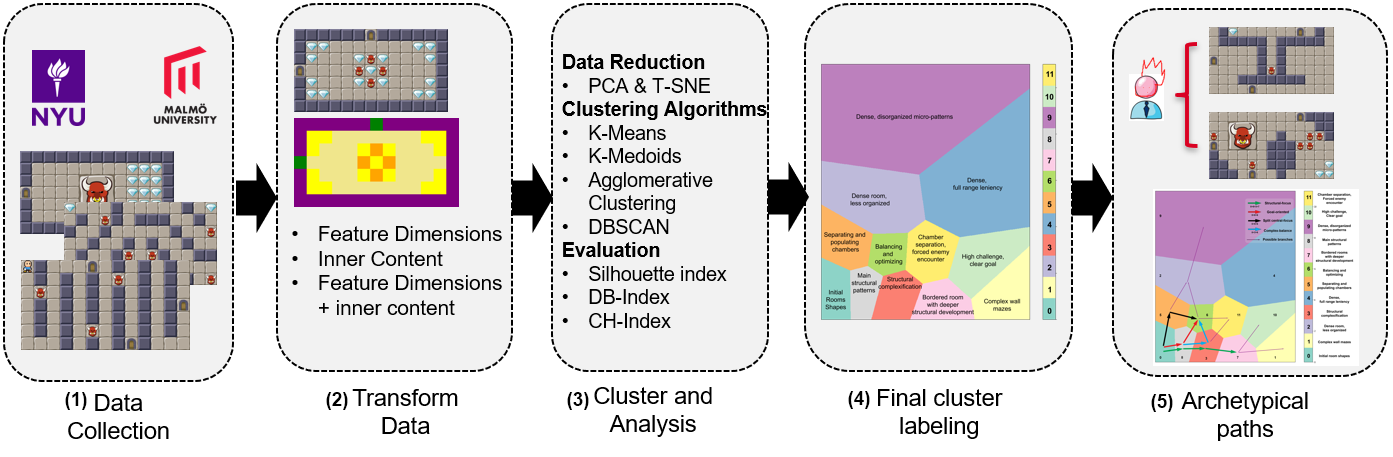
\includegraphics[width=\textwidth]{figures/process-steps.png}}
\caption{The stages of the design style clustering development: (1) Data was first collected through two user studies. (2) Then, using the design sequences, the data was processed into five different datasets, one using the room images, a second using the tiles information, and three using tabular information. (3) A data reduction technique was applied to different datasets, and then they were clustered and internally evaluated. (4) The clusters were formed, picked from the best performing methods, and labeled based on the data points within each cluster. The cluster were evaluated by visualizing how a typical design session traverse the various clusters, and K-Means (K=12) was chosen as the final approach. (5) Finally, using this final approach all the sequences were clustered and archetypical paths were identified.%(5) The final approach,  K-Means (K=12) was evaluated by visualizing how a typical design session traverse the various clusters. Finally, the sequences were clustered by the final approach and archetypical paths were identified.
} \label{p6fig:approach-steps}
\end{figure*}

\begin{figure*}[t]
\centerline{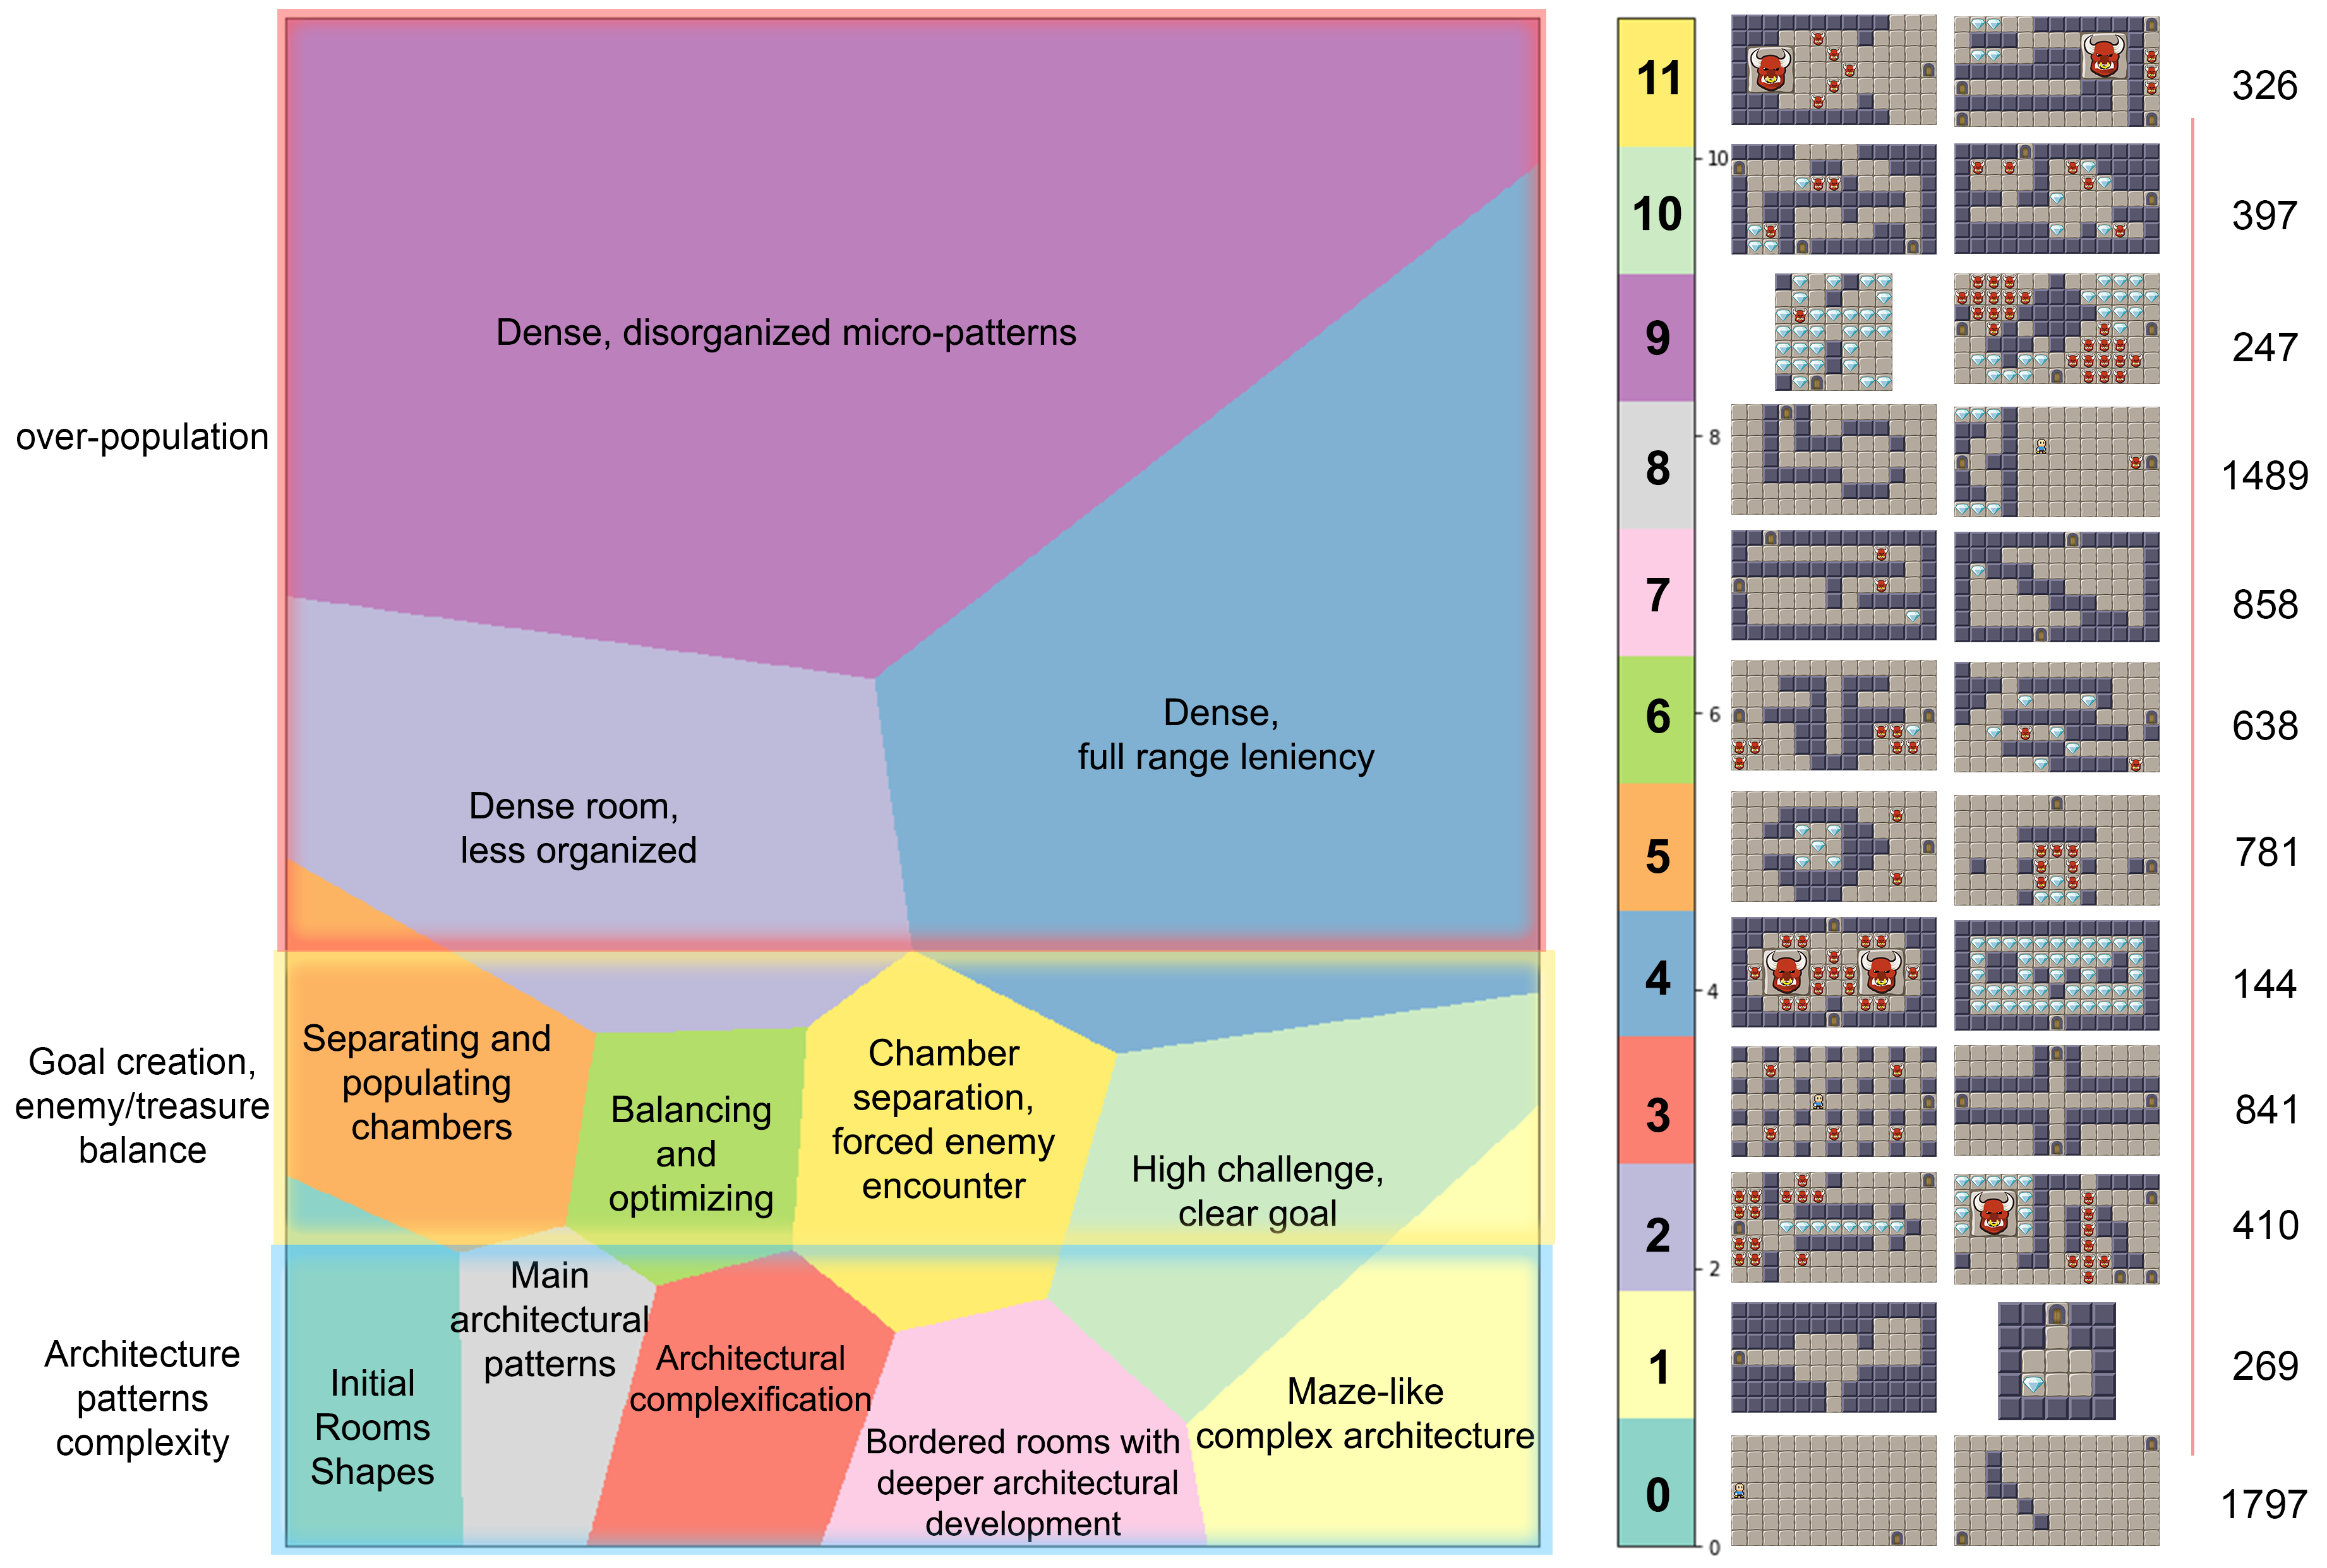
\includegraphics[width=\textwidth]{figures/final-cluster.png}}
\caption{Best resulting cluster set. K-Means (K=12), using the \textbf{Tiles} Dataset. While it scores slightly less in the internal indices that other setups, a qualitative analysis successfully gives us more granularity by subdividing the main bottom clusters, to label and cluster the design process of designers. Sample rooms belonging to each cluster are displayed on the right, next to the total number of rooms in the cluster.} \label{p6fig:all-clusters}
\end{figure*}

% \begin{figure*}[b]
% \centerline{\includegraphics[width=13cm]{figures/representative cluster-steps.png}}
% \caption{Examples of a step by step edition sequence of a design session and it's clustering. To the left, we present the actual sequence and steps of one of the rooms in the dataset and to the right is the actual trajectory of the design in the cluster space. Numbered and in black, it is shown how each step of the design process is clustered by our approach} \label{p6fig:paths-designers}
% \end{figure*}

% \begin{figure}[h]
% \centerline{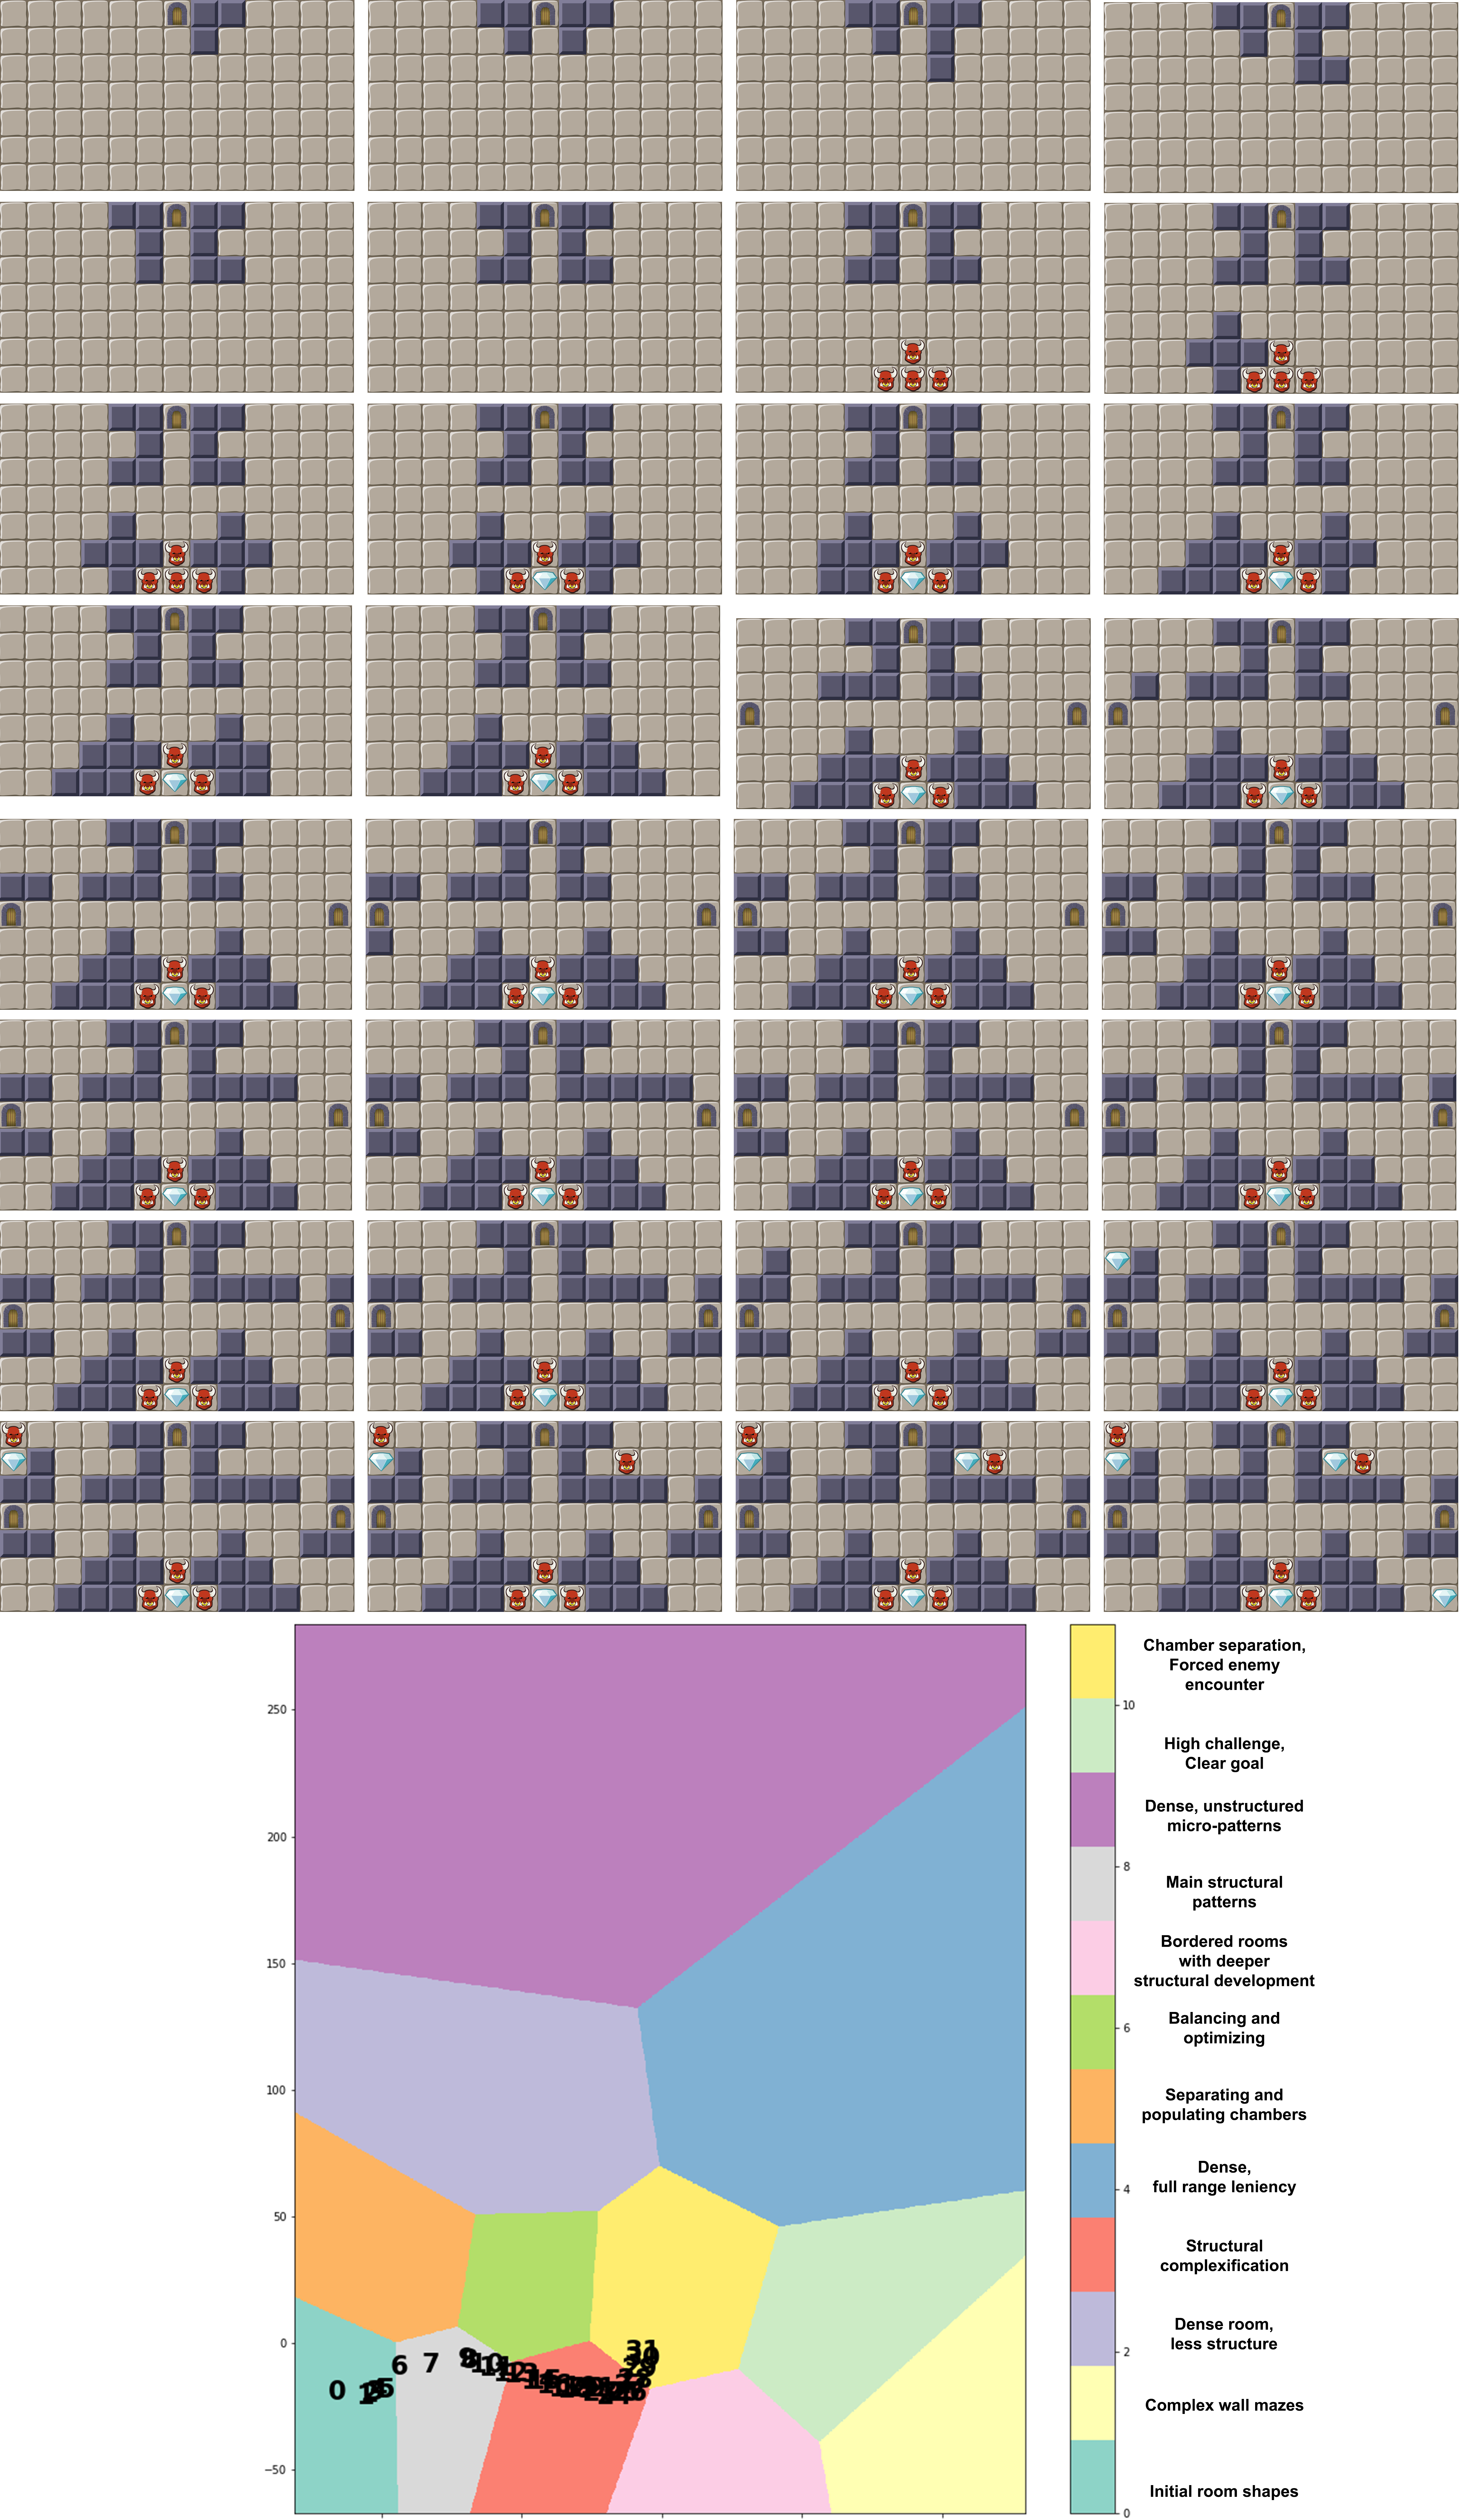
\includegraphics[width=8cm]{figures/representative-cluster-steps-alter.png}}
% \caption{Example of a step by step edition sequence of a design session and it's clustering. At the top, we present the actual sequence and steps of one of the rooms in the dataset, in a $4\times7$ grid, starting at the top left with the first edition. At the bottom, it is the actual trajectory of the design in the cluster space. Numbered and in black, it is shown how each step of the design process is clustered by our approach} \label{p6fig:paths-designers}
% \end{figure}

\begin{figure*}
\centerline{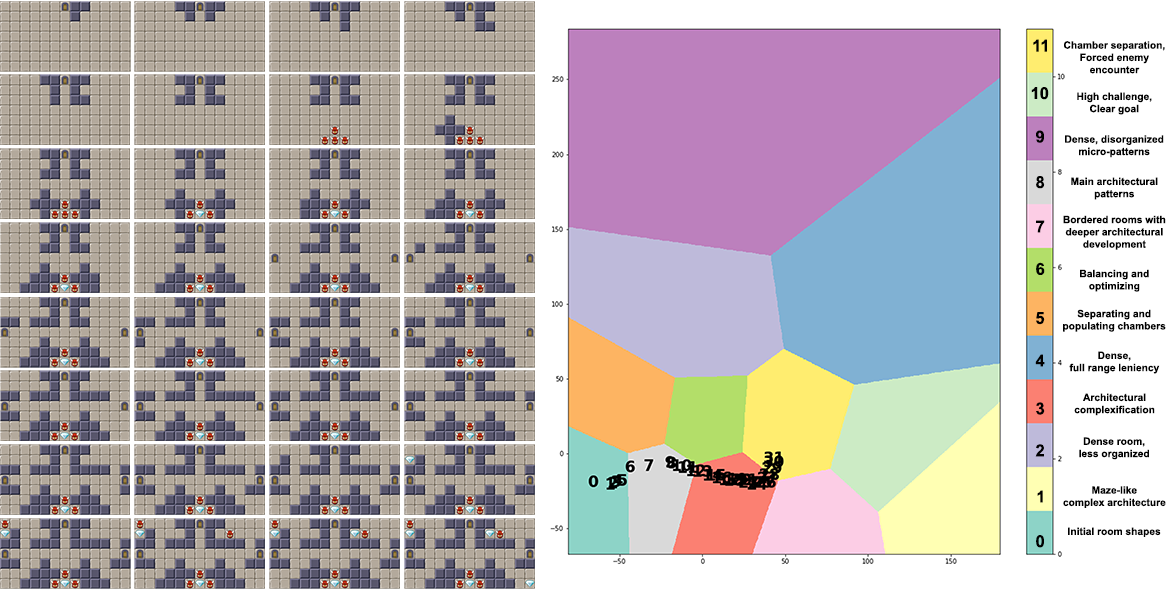
\includegraphics[width=\textwidth]{figures/representative-clusters-small.png}}
\caption{Example of a step by step edition sequence of a design session and it's clustering. At the left, we present the actual sequence and steps of one of the rooms in the dataset, in a $4\times7$ grid, starting at the top left with the first edition. At the bottom, it is the actual trajectory of the design in the cluster space. Numbered and in black, it is shown how each step of the design process is clustered by our approach} \label{p6fig:paths-designers}
\end{figure*}

This paper presents an approach and fundamental steps towards the implementation of designer personas: an analysis of designer style clustering to isolate archetypical paths that can be later be used to build ML surrogate models of archetypal designers. Such models would adapt to the dynamic designer during the mixed-initiative creative process by being placed in the solution space, allowing the designer to traverse such space of models as she drifts through the many dimensions of her creative process.

The proposed system builds on top of EDD's Designer Preference Model and preliminary results \citepsixth{p6Alvarez2020-DesignerPreference}, expanding it to classify the designers' designs based on clusters developed using previously hand-made design sequences by expert and non-expert designers. Figure \ref{p6fig:approach-steps} illustrates our approach in five sequential stages, from data collection to experimentation and results. The first four stages are explained in the following subsections, whereas Section~\ref{p6section:results} shows the experimental results.

\subsubsection{Data Collection}

We conducted two user studies where participants were tasked with freely designing a dungeon in EDD and the rooms that compose it with no further restrictions, using all the available tiles i.e. floor, wall, treasure, enemy, and boss tiles. All participants were introduced to the tool before the design exercise. User-generated data was gathered during the complete design session, creating a new data entry every time the designer edited the dungeon. In total, we had $40$ participants, $25$ of these (i.e. NYU participants) were industry or academic researchers within the Games and AI field, and the other $15$ (i.e. MAU participants) were game design students. This resulted in a diverse dataset composed of $180$ unique rooms like the ones depicted in Figure~\ref{p6fig:approach-steps}, that was pre-processed and clustered in the subsequent stages. 

\subsubsection{Dataset pre-processing}

From the $180$ unique rooms, we extracted and used the edition sequence of each of the rooms, from their initial design to the more elaborated end-design, to compose a richer dataset that could capture the design process of a designer rather than focusing on the end-point. Through this, we ended up using $8196$ data points in our dataset.
%just the end-point. We ended up using $8196$ rooms
Moreover, five different copies of the dataset were created to analyze and compare the performance of the clustering stage using the following image pre-processing methods:

\begin{enumerate}
\setcounter{enumi}{0}
    \item \textbf{Room:} No pre-processing. Room images are fed into the next stage as they were created by the designer, with a resolution of $1300\times 700\times3$, corresponding to width, height, and RGB ($3$ color channels).
    
    \item \textbf{Tiles:} Each room tile type is mapped to a single-color pixel and the rooms are simplified to a pixel-tile based representation, as shown in the second stage of Figure \ref{p6fig:approach-steps}. The dimensions are downscaled to $13\times 7\times3$.
    %Each room tile is simplified to a single-color pixel, as shown in the second stage of Figure \ref{p6fig:approach-steps}, downscaled to $13\times 7\times3$.
    
    \item \textbf{Dimensions:} Each room is described by its five IC-MAP-Elites feature dimension values, excluding the similarity scores: \textsc{Linearity}, \textsc{Leniency}, \textsc{\#MesoPatterns}, \textsc{\#SpatialPatterns}, and \textsc{Symmetry}. A complete description of these features can be found in~\citepsixth{p6Alvarez2020-ICMAPE}.
    
    \item \textbf{Inner Content:} Each room is described by $12$ values, related to the count, sparsity, and density of the enemy, treasure, floor, and wall tiles contained in it.
    
    \item \textbf{Combined:} A combination of the \textbf{Dimensions} and \textbf{Inner Content} methods.
\end{enumerate}

\subsubsection{Clustering and Analysis}

To run all setups, data reduction algorithms, clustering algorithms, and do the internal evaluation of the clusters, we used scikit-learn machine learning toolset~\citepsixth{p6scikit-learn}. To obtain the best set of clusters, we ran different setups with the above datasets. The data was reduced to two meaningful dimensions with two different data reduction algorithms, Principal Component Analysis (PCA) and T-Distributed Stochastic Neighbor Embedding (T-SNE). For both data reduction algorithms, we fit the algorithms with each individual dataset, setting to two principal components and in the case of T-SNE using PCA as initializing algorithm, and transforming the data into a new dataset \emph{pca\_dataset} and \emph{tsne\_dataset} per dataset. Each two-dimensional point in the new datasets represents a step in the sequences described above.%Likewise, for the T-SNE, we fit the algorithm with each individual dataset, setting the parameters to two principal components and using PCA as initializing algorithm, and then transformed the data into a new dataset \textit{tsne_dataset} per dataset.

Moreover, all the resulting datasets were then clustered using \textsc{K-Means, K-Medoids, Agglomerative clustering}, and \textsc{DBSCAN}. K-Means was initialized using the standard k-means++ implemented in scikit-learn, which initialize all centroids distant from each other. K-Medoids was initialized similarly, using the standard k-medoids++, and tested using the \emph{cosine}, \emph{euclidean}, and \emph{manhattan} distances. Agglomerative clustering is a hierarchical clustering approach using a bottom-up approach implemented in scikit-learn using four different linkage criteria for comparing data points: \emph{Ward}, \emph{Complete}, \emph{Average}, and \emph{Single}. Finally, DBSCAN cluster points based on density separated by low-density areas; thus, DBSCAN automatically finds $k$ based on two parameters, $\epsilon$ describing the maximum distance between points and \emph{min\_samples} describing the minimum amount of samples within a group to be considered a cluster. K-Means, K-Medoids, and Agglomerative clustering were tested using multiple $K$ values ranging from 3 to 13, and DBSCAN was tested with several $\epsilon$ values ranging from 0.3 to 1.0, and \emph{min\_samples} ranging from 2 to 9.

%, testing with $K$ values ranging from 3 to 13 for the first three ones, and several $\epsilon$ values for DBSCAN.

%testing different minimum distance between data points ($\epsilon$) and the minimum amount of data points within a cluster to be considered a dense region for DBSCAN.

Since we lack a labeled dataset (i.e. ground truth) for cluster validation, we evaluated the results from all setups using the internal indices below, as well as manually inspecting the rooms composing the resulting clusters.

%Since in our approach lacks a labeled dataset (i.e. ground truth) for cluster validation, 

\begin{itemize}
\item \textbf{Silhouette Score:} The Silhouette Score shows how similar a data point is to the cluster it is associated with, through calculating the difference between the $\overline{distance}$ from the point to the points in the nearest cluster and the $\overline{distance}$ to the points in the actual cluster. The value is bounded from -1 to +1, with values closer to +1 indicating a good separation of the clusters, and closer to -1 meaning that some points might belong to another cluster.
\item \textbf{Davies-Bouldin Index:} The DB-index is the ratio between the within-cluster distances and between-clusters distances. With this, we can have an insight into the average similarity of clusters with their closest cluster. The value is bounded from 0 to +1, with values closer to 0 relate to clusters that are farther apart from each other and less dispersed, thus, this index is more crucial when we have more dense representations.
\item \textbf{Calinski-Harabasz Index:} The CH-index is another index related to the density of the clusters and how well separated they are. The score is the ratio between the within-cluster dispersion (compactness) and the between-cluster dispersion (separation). The CH-index is positively unbounded, and the higher the score the better.
\end{itemize}

\subsubsection{Cluster Labelling}

\begin{table}
\begin{center}
{\caption{Best performing setups based on their internal validation and visualization of clustered data points.}\label{p6table:setups}}
\resizebox{0.9\textwidth}{!}{
\begin{tabular}{ccccccc}
\hline
\rule{0pt}{12pt}
Algorithm&Data&K&$\Diamond$&$\Box$&$\bigtriangleup$ 
\\ 
\hline
\\[-6pt]
K-Means & Tiles-PCA & 9 & 0.43 & 0.73 & 9438.233 \\ 
K-Means & Tiles-PCA & 12 & 0.41 & 0.77 & 9436.928 \\
K-Means & Dimensions-PCA & 12 & 0.43 & 0.73 & 7738.343 \\
Agglomerative single & Combined-PCA & 6 & 0.51 & 0.43  & 38.833 \\ 
Agglomerative avg. & Dimensions-PCA & 6 & 0.44 & 0.67 & 3463.567 \\ 
\hline
\\[-6pt]
\multicolumn{6}{l}{$\Diamond$ Silhouette Score\ \
$\Box$ Davies Bouldin Index\ \
$\bigtriangleup$ Calinski-Harabasz Index}
\end{tabular}
}\end{center}
\end{table}

Table~\ref{p6table:setups} shows the best performing setups according to their internal indices scores. The clusters in these setups were manually inspected in order to detect the qualitative features that better define them. 

When using the \textbf{Dimensions} and \textbf{Combined} datasets, the clusters do perform good, if not better, in certain indices than when using the \textbf{Tiles} dataset. However, when analysing the resulting setups, they were missing a clearer relation between the clustered rooms, which was exacerbated when analysing sequences and paths on these setups, where they missed continuity between clusters.

Conversely, given that we are creating tile-based rooms and dungeons, the features were more representative for the \textbf{Tiles} dataset, which when used, generally performed well in the evaluated internal indices, and the produced clusters meaningfully separate the data. Further, as it will be presented in Section \ref{p6section:results}, when clustering sequences and analyzing the cluster path of the designs, there exist a continuity between designs that supports its usability. Figure \ref{p6fig:all-clusters} shows the best-resulting cluster set found among all the experiments run.



% As expected, the \textbf{Tiles} dataset generally performed well in the evaluated internal indices, and the produced clusters meaningfully separated the data.
% better information and were meaningfully group together.  relation each of the features have with 

% As expected, the \textbf{Tiles} representation have good results across the 3 indices, 

% JOSÉ: I leave it here waiting for the final results from Alberto

%Moreover, We noticed that the agglomerative approach results in very specific clusters alongside a quite broad cluster consisting of unrelated data points, regardless of the $K$ used. These setups scored well in the different indices but fail to accurately partition the space in relevant groups.

%Moreover, there are recurrent clusters between the different setups but when using more clusters like in figure~\ref{p6fig:all-clusters} (b), we can have more granularity when partitioning the space, improving the separation of more related data points. In figure~\ref{p6fig:all-clusters}(b) we present several rooms that have been clustered together matching the labeling of the clusters. In the figure, there is a clear correlation between the designs and the labels of their respective cluster, and an interesting continuity between the final clusters.

% In Figure~\ref{p6fig:all-clusters}, we present the final and selected approach for clustering room styles using K-Means (K=12) and the \textbf{Tiles} dataset reduced with the PCA algorithm. To the right, next to each color in the legend, we have different representative rooms that belong to the clusters, in their respective color, and have been clustered together. Furthermore, besides the local relation between clusters, there exists a layered division among group of clusters in the y-axis, where the bottom clusters relate more to architectural pattern complexity, from very empty rooms to mazes. The middle clusters focus on populating the rooms with enemies and treasures, creating the actual goals of the room and balancing the challenge. Finally, the top clusters are composed of dense rooms where the enemy and treasure addition do not necessarily need to follow any clear objective. 


% The clusters's label are plotted on top of each of the clusters, describing in general, the content that is within them. These cluster 

In the figure, we have plotted on top of the clusters the labels describing in general, the content that is within them. The following is a description of the clusters and the rooms that were clustered together:

\textbf{0. Empty-Initial rooms:} %This cluster contains $1797$ data points, and 
This cluster relates mostly to the initial designs made by the designers. These designs are from completely empty rooms to initial work-in-progress structures.

\textbf{1. Maze-like complex architecture:} This cluster to the extreme of the architectural patterns complexity layer, relates to more highly-linear, confined and maze-like rooms.% with more structure on what is possible. %The cluster contains $269$ data points.

\textbf{2. Dense, less organized:} This cluster contains rooms that still have a certain objective but are moving towards more disorganized distributions of micro-patterns in relation to their density. %This cluster contains $410$ data points.

\textbf{3. architectural complexification:} %This cluster contains $841$ data points, and 
This cluster relates mostly to the complexification of wall structures by having dense wall chunks, representative architectural patterns, or symmetrical patterns.

\textbf{4. Dense, full range leniency:} Focusing on density as the other two clusters within the same layer, this cluster relates to rooms that are in the full range of leniency from very rewarding, treasure rooms to very challenging boss rooms. %This cluster contains $144$ data points.

\textbf{5. Separating and populating chambers:} This cluster relates to the process of separating rooms into distinct chambers, focusing on the center of the room, and starting to populate rooms with enemies and treasures. %The cluster contains $781$ data points.

\textbf{6. Balancing and optimizing:} This cluster contains a mix between corridors and chambers within rooms with a focus on balancing rooms and optimizing their design towards certain goals. %The cluster contains $638$ data points.

\textbf{7. Bordered rooms with deeper architectural development:} This cluster relates mostly to rooms with an added wall border by the designer, and where the focus is to shape chambers and develop more visual structures.

\textbf{8. Main architectural shapes:} Similar to other clusters within the same layer, this cluster relates to the development and definition of main architectural patterns that are somewhat symmetric.

\textbf{9. Dense, disorganized micro-patterns:} This cluster clusters the extreme rooms that contain a high density of tiles, other than floor-tiles, without a clear structure or objective for the player.

\textbf{10. High challenge, clear goal:} This cluster relates to well-shaped rooms with clear wall structures and goals, towards more challenge. 

\textbf{11. Chamber separation with forced enemy encounter:} This cluster relates to rooms that are in the process of a clear segmentation into corridors and chambers, and that enforce to some extent, enemy encounters for the player. 

Furthermore, besides the local relation between clusters, the clusters are implicitly divided in three layers on the Y-axis. From bottom to top, (a) architectural patterns complexity, relating to clusters composed of rooms with clearer or complex shapes done with walls, from empty rooms to mazes. (b) Goal creation, enemy/treasure balance, with clusters comprehending the strategic addition of enemies and treasures to establish objectives in the room for the player. In terms of EDD, these rooms are composed of more meso patterns. And (c), over-population, which relates to clusters filled with less organized and dense rooms where the enemy and treasure addition do not necessarily need to follow any clear objective. Identifying the designer in such layer, and the path they have taken to get there could show meaningful information in the design process. For instance, the intentions of the designer, in what phase of the design process she is at the moment i.e. trying the tool or observing how the tool reacts or scraping her current goal towards a new goal within the room. 

% \begin{enumerate}
% \setcounter{enumi}{-1}
% \item[0] \textbf{Empty/Initial rooms:}
% \item \textbf{Complex wall mazes:} 
% \item \textbf{Dense, less structure} 
% \item \textbf{Structural complexification:} 
% \item \textbf{Dense, full range leniency} 
% \item \textbf{Separating and populating chambers:} 
% \item \textbf{Balancing and optimizing rooms:} 
% \item \textbf{Bordered rooms with deeper structural development:}
% \item \textbf{Development of main structural shapes:} 
% \item \textbf{Dense, unstructured:} 
% \item \textbf{Challenging rooms with clear goal:} 
% \item \textbf{Chamber separation with forced enemy encounter:} 
% \end{enumerate}



\begin{figure*}[t!]
\centerline{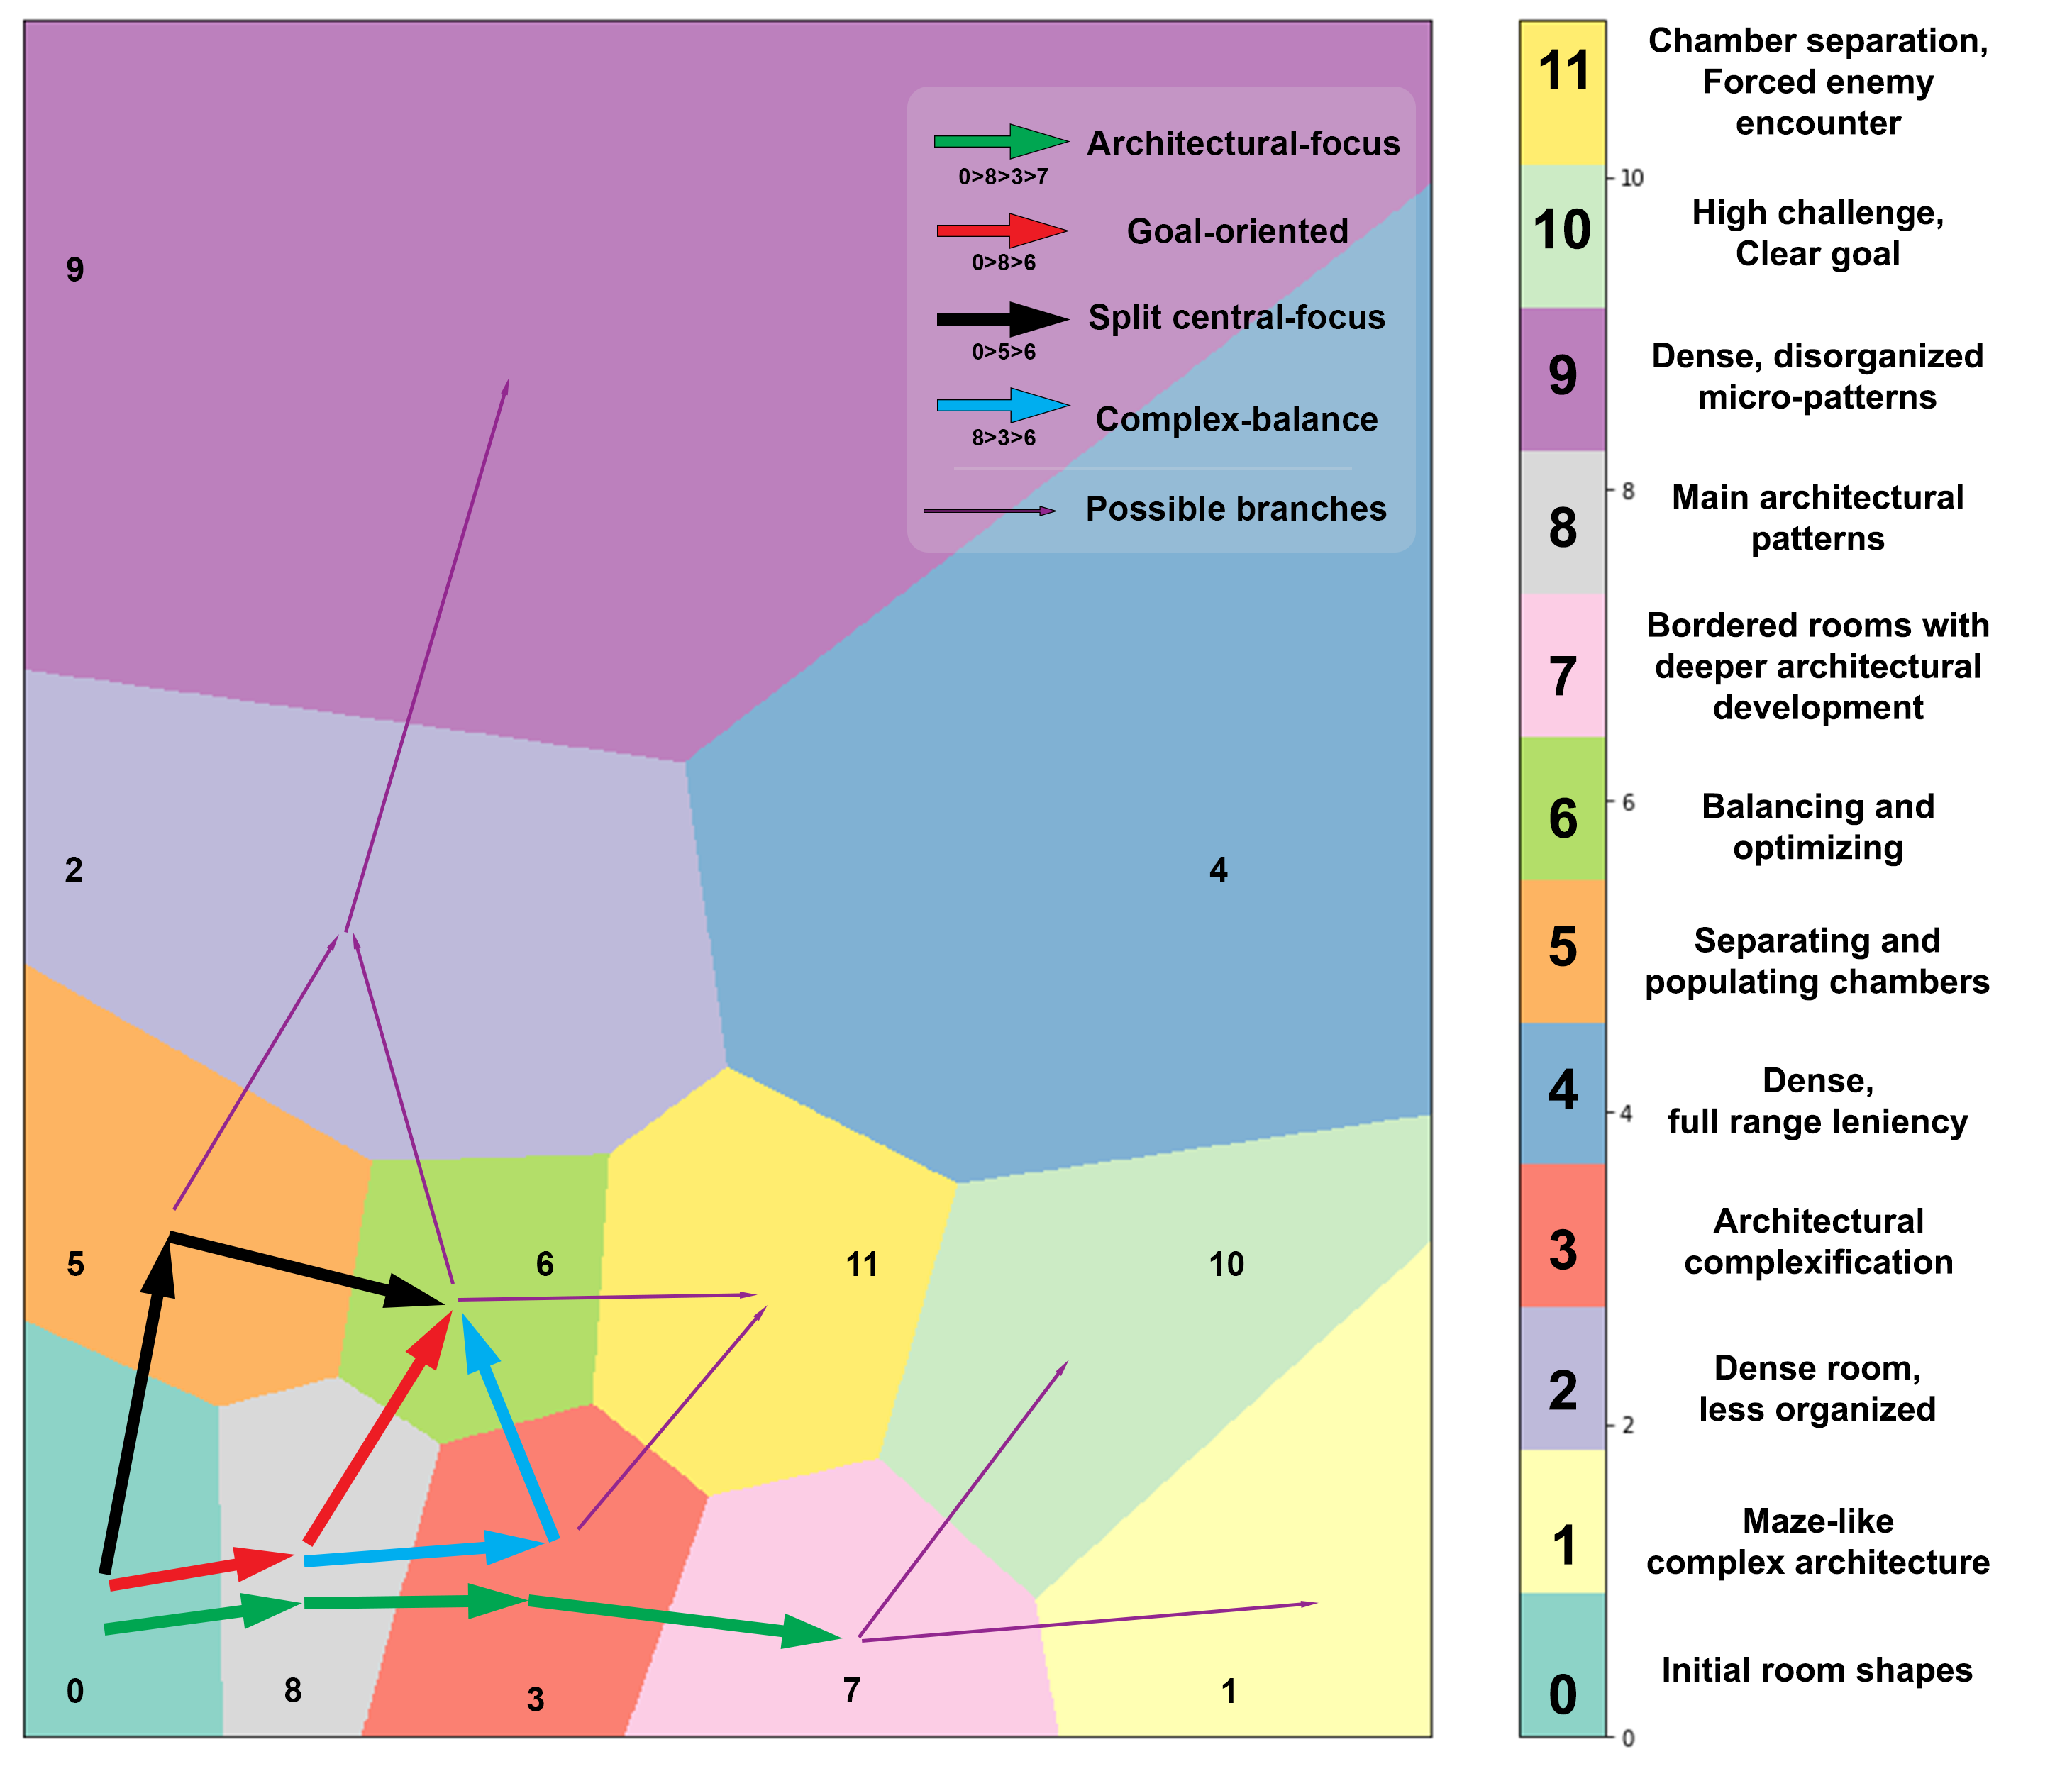
\includegraphics[width=\textwidth]{figures/resulting-paths-FINAL.png}}
\caption{Final and common designer trajectories. With thick arrows it is presented the archetypical paths, calculated using the frequencies of subsequences from $180$ diverse rooms. Each color represent a unique trajectory; with green the \textsc{Architectural-focus}, with red the \textsc{Goal-oriented}, with black the \textsc{Split central-focus}, and with blue the \textsc{Complex-balance}. Finally, thinner purple arrows extending from clusters traversed by the archetypical paths show the multiple possible branches that an archetypical path can deviate or extend to.} \label{p6fig:finalPaths}
\end{figure*}

% \begin{figure*}[t]
% \centerline{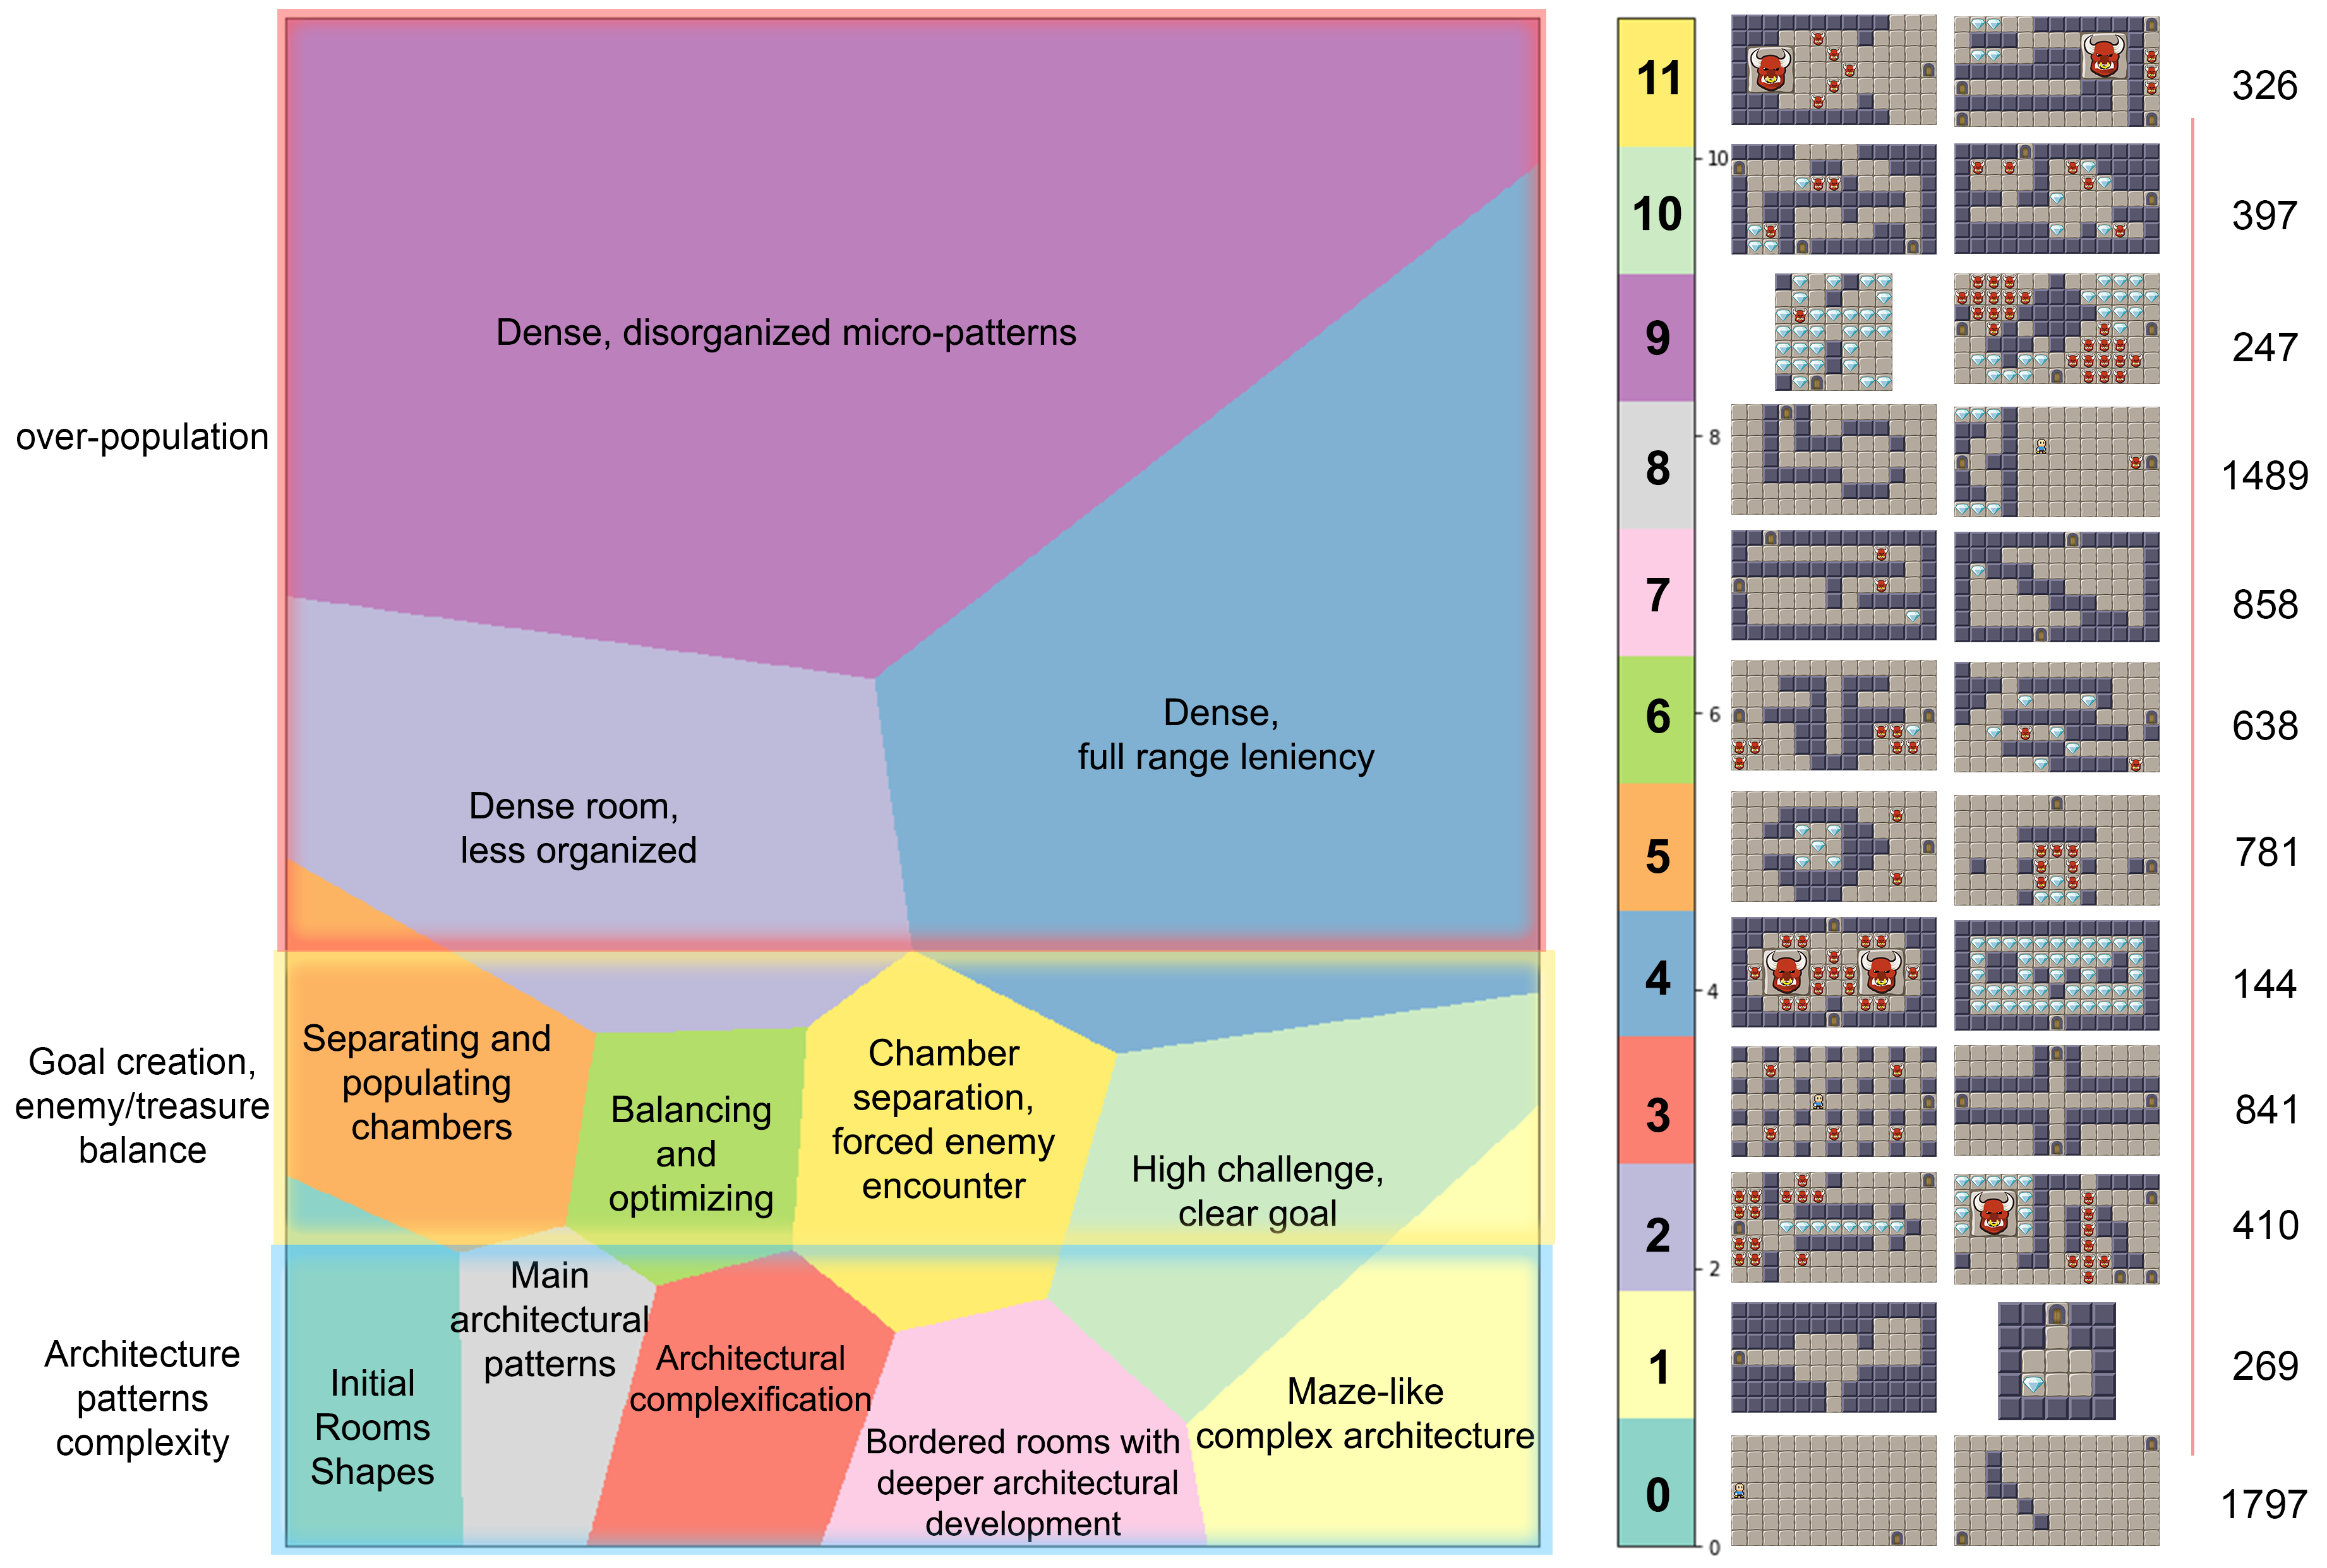
\includegraphics[width=16cm]{figures/final-cluster.png}}
% \caption{Best resulting cluster sets. (a) is K-Means (K=9), and (b) is K-Means (K=12), both are using the \textbf{Tiles} Dataset. While (b) performs slightly worst in the internal indices, when inspecting the qualitative features, it successfully subdivides the main bottom clusters which grants us with more granularity to label and cluster the design process of designers.} \label{p6fig:all-clusters}
% \end{figure*}

% \begin{figure}[t]
% \centerline{\includegraphics[width=8cm]{figures/cluster-figure-updated.png}}
% \caption{Overview of how the design style clustering would be used and integrated into the evaluation of the suggestions provided to the user. %is used and integrates into the evaluation of the suggestions provided to the user.
% } \label{p6fig:cluster}
% \end{figure}

% \begin{figure}[t]
% \centerline{\includegraphics[width=8cm]{figures/all_clusters.png}}
% \caption{All the selected clusters to be labeled and analyzed. In order, each of the clustering approaches correspond to the setups presented in table~\ref{p6table:setups}. (e) Shows extra information on the designs that were clustered together, and which were used to label the respective cluster.} \label{p6fig:all-clusters}
% \end{figure}

% \begin{figure}[b]
% \centerline{\includegraphics[width=8cm]{figures/hand-made-clusters.png}}
% \caption{Example of hand-made room designs used to create the clusters. only (a) and (b) belong to the same clusters} \label{p6fig:handMadeClustered}
% \end{figure}

% \begin{figure*}[t]
% \centerline{\includegraphics[width=18cm]{figures/approach_steps.png}}
% \caption{Rooms at generation $2090$ targeting Number of spatial-patterns (X) and Symmetry (Y). Each cell displays (top-right) the fitness of the optimal individual in its related feasible population. }
% \label{p6figs:approachSteps}
% \end{figure*}

% \begin{figure}[t]
% \centerline{\includegraphics[width=8cm]{figures/cluster-figure-updated.png}}
% \caption{Example of a figure caption.}
% \label{p6fig:implementationClusters}
% \end{figure}
% Please add the following required packages to your document preamble:
% \usepackage{graphicx}
\begin{table*}[t]
\resizebox{\textwidth}{!}{%
\begin{tabular}{|l|lllllllllll|l|}
\hline
AIs  & Len       & Lin       & Meso      & Spatial   & Symmetry  & $W_{dens}$ & $W_{spar}$ & $E_{dens}$ & $E_{spar}$ & $T_{dens}$ & $T_{spar}$ & Steps       \\ \hline
AIv1 & 0.56±0.07 & 0.91±0.02 & 0.15±0.05 & 0.35±0.1  & 0.43±0.11 & 0.27±0.09  & 0.21±0.05  & 0.24±0.07  & 0.22±0.05  & 0.37±0.13  & 0.36±0.11  & 39.25±6.38  \\
AIv2 & 0.62±0.09 & 0.92±0.02 & 0.13±0.07 & 0.41±0.11 & 0.35±0.18 & 0.26±0.08  & 0.19±0.03  & 0.27±0.06  & 0.32±0.05  & 0.28±0.09  & 0.3±0.1    & 84.31±14.85 \\
AIv3 & 0.57±0.08 & 0.91±0.01 & 0.12±0.05 & 0.34±0.09 & 0.35±0.12 & 0.21±0.05  & 0.15±0.01  & 0.3±0.06   & 0.35±0.06  & 0.34±0.07  & 0.37±0.05  & 76.75±17.02 \\ \hline
\end{tabular}%
}
\caption{Summary of the created rooms filtered by the AI version used. The first five values relates to the MAP-Elites dimensions, then the fitness of the rooms, the density and sparsity values for wall (W), enemies (E), and treasures (T), and finally the avg. steps taken to design a room.}
\label{tab:AIavgValues}
\end{table*}

\subsection{Experiment Setup}

We conducted a user study to explore the user experience of using different levels of AI agency, the different design characteristics, and the relationship between the human designer and the AI. We collected both quantitative data on the AI's impact on the co-designed end product and qualitative data through think-a-loud and semi-structured interviews regarding the users' experience when interacting with the AI. The interview structure is inspired by the pyramid model, meaning the interviews will begin with specific questions, and gradually have more open questions, which naturally allows for a discussion towards the end. This model is chosen to support the variation of subjects the interview is desired to cover, as well as support natural transitions between the questions and their openness. The questions and user study procedure can be found in Appendix A. 

%The interviews are semi-structured, meaning it includes both closed and more open questions, and depending on the discussion and answers, some questions might be omitted.

% We collected quantitative data regarding what impact the AI had on the co-designed end product, and how the human designer interacted with the AI's contributions. Likewise, we collected qualitative data through recorded think-aloud observations and semi-structured interviews regarding the users' experience, and possibly catch certain remarks of frustration or appreciation of their digital colleague that can be valuable for the discussion of the relationship between the co-creators. 


%We collected the following data:

%\begin{itemize}
%    \item \textbf{Audio Recordings:} 
%\end{itemize}

Eight participants tested our tool with game design and level design experience. One participant was a professional game designer with eight years of professional experience (first participant), and seven participants were third-year Game Development students. They all had an individual digital session, where we shared our screen, and they took remote control to conduct the study. Participants accepted to participate, signed consent forms, and then received a short introduction describing the experiment and its steps. The participants were then asked to design two contiguous rooms in a dungeon, repeating this process for each of the AI variants and expressing their design decisions verbally whenever they felt like it. After using the tool, the participants were interviewed, focusing on and covering an overarching understanding of the user experience, particularly in terms of creativity and interaction with the AI.

% the relationship that occurs between the AI and human designer (See Appendix B). 

For all the sessions, human designers could place up to 12 tiles, and the AI could place as many tiles as the human placed. The AI could contribute only in a rectangular area surrounding the tiles the human designer recently contributed with, including a margin of 1 tile. This choice is made to support a responsive and collaborative behavior of the AI that builds on the human designer's contribution.


% The locations available for the AI to contribute in for each turn are limited to a rectangular area surrounding the tiles the human designer recently contributed with, including a margin of 1 tile. This choice is made to support a responsive and collaborative behavior of the AI that builds on the human designer's contribution.

% The margin for the contribution area is set to 1, as it was found during experimentation that any margin bigger than this is likely perceived as the AI contributing to other areas than the ones the human is focused on, because of the default size of the room being relatively small.

%  as this enables the designer to contribute with an adequate amount of tiles during their turn and create representable structures

% The rooms produced during the user study are displayed in Figure 6, 7 and 8. Rooms with red borders are infeasible, meaning there are unreachable tiles. The UI displays a warning when this happens, and the AI can repair this during its turn, however the resulting rooms that are infeasible are a result of the human designer creating unreachable areas, and then immediately selecting to go to the World Editing view, before pressing "End Turn". 
% Each participant created two rooms for each version of the AI. Participant 1 created Room 1 and Room 2 for all version, Participant 2 created Room 3 and Room 4 for all version, etc. All of the participants had the option to adjust the sizes of the rooms in the World Editing view before entering the Room Editing view, however none of them did, and therefore all of the resulting rooms are of the default size. The designer also has the option to change the location of the hero and the doors. The location of the hero was only moved twice in all of the session, and the doors where never moved. 






%, the participant will take part in an interview. The questions, and their order, are planned out and designed to cover an overarching understanding of the user experience, in particular in terms of creativity, and the relationship that occurs between the AI and human designer (See Appendix B). 




%The participants were asked to repeat this for each of the AI-initiatives. was asked to repeatEach pair of room 

% then asked to complete three tasks, each regarding

%The users were then asked to complete three tasks that covered the tool's functionality and the AI-initiatives, respectively for each task. The tasks were 


%and different approaches to creating quests. The tasks were to 1) manually create a quest, 2) automatically create a quest, and 3) create a quest through mixed-initiative. They were also asked to create a dungeon that suited their preferences and objectives before creating quests. The questionnaire consisted of 17 closed-ended questions, and the rest were open-ended. The interview began with a questionnaire with six questions about the users' background and experience within game development and finish with questions about their experience and opinions on the tool. Both the questionnaire and interview followed guidelines described by



%The participants used the tool



\subsection{Conclusions}



% \begin{itemize}
%     \item Discussion on what does this archetypical design trajectories mean?
%     \item how to use them? next steps into integrating this into a system. To use this in a search-based approach as objectives for the generation to move towards the directions where (according to our archetypical design trajectories) the designers will move towards in their design process. Perhaps I could also bring the discussion from the workshop-paper for HC-AI.
%     \item discussion on creativity? is the output or the process where the actual creativity is outputted? Compare using end-design clustering to using sequences to cluster.
%     \item Discussion on how PCGRL relates to this type of work? --> Perhaps this is something for the background instead.
% \end{itemize}{}


% This paper presents a step towards designer modelling in a MI-CC environment by providing an implementation of designer personas as archetypical trajectories through style space, as a means to characterize several representative and frequent design styles together. 

%This paper presents a novel approach and meaningful steps towards designer modeling in an MI-CC environment. By providing an implementation of designer personas as archetypical trajectories through style space, we show that 

This paper presents a novel approach and meaningful steps towards designer modeling through an experiment on archetypical design trajectories analysis in an MI-CC environment. Through this, we characterize several representative design styles as designer personas. We have first run and compared several clustering setups to find the best partitioning of the design style using the edition sequences of the collected $180$ unique rooms, ending in $8196$ data points, and resulting in a set of twelve cohesive, coherent, and meaningful clusters. We have then mapped these $180$ design sequences in terms of these clusters, applying frequent sequence mining to find four frequent and unique designer styles, with related common sub-styles. As a result, we have presented a roadmap of design styles over a map of data-driven design clusters. 

%This paper presents a step towards designer modeling through an experiment on archetypical design trajectories analysis in an MI-CC environment, as a means to characterize several representative design styles as designer personas. We have first run and compared several clustering setups to find the best partitioning using the edition sequences of the collected $180$ unique rooms, ending in $8196$ data points, and resulting in a set of twelve cohesive, coherent, and meaningful clusters. We have then mapped these $180$ design sequences in terms of these clusters, applying frequent sequence mining to find four frequent unique designer styles, with related common sub-styles. As a result, we have presented a roadmap of design styles over a map of data-driven design clusters. %The examples in Figure \ref{p6fig:archetypical-examples}, help us to clarify 

%  namely the \textsc{Designer Personas}

% Our work draws on the ideas, concepts, and goals and concepts proposed by Liapis et al. when introducing the Designer Modeling as a model to capture multiple designer's processes. A prototype of such was implemented in the sentient sketchbook~\citepsixth{p6Liapis2014-designerModelImpl}, where it is proposed the use of interactive evolution by biasing the search space in favor of hand-crafted features of the design. we propose an alternative and novel route to designer modeling through clustering the design space and the room style based on the collected data. Moreover, we differ as well on the type of level design, being the sentient sketchbook a tool for strategy games~\citepsixth{p6liapis_generating_2013}, while EDD a tool for adventure and rogue-like games~\citepsixth{p6Alvarez2020-ICMAPE}. These differences strengthen the importance and usefulness of designer modeling, and highlight the holistic and generic properties of this designer-centric perspective.

Designer modeling was proposed as an approach to capture multiple designer's processes to create a better workflow by Liapis et al.~\citepsixth{p6Liapis2013-designerModel}, and our work draws on many of their ideas, concepts, and goals. Furthermore, a prototype of such was implemented in the sentient sketchbook~\citepsixth{p6Liapis2014-designerModelImpl}, where it is proposed different approaches to model style, process, and goals based on choice-based evolution and the designer's current design to adapt the provided suggestions accordingly. We propose an alternative route to designer modeling through clustering the design space and the room style based on the collected data. Moreover, we differ in the type of level design, being the sentient sketchbook a tool for strategy games~\citepsixth{p6liapis_generating_2013}, while EDD is a tool for adventure and rogue-like games~\citepsixth{p6Alvarez2020-ICMAPE}. These differences strengthen the importance and usefulness of designer modeling and highlight the holistic and generic properties of this designer-centric perspective and its possibilities.

% Designer modeling in computer-aided design tools was proposed by Liapis et al.~\citepsixth{p6Liapis2013-designerModel} as an approach to capture multiple designer's processes to create a better workflow, and a prototype of such was implemented in the sentient sketchbook~\citepsixth{p6Liapis2014-designerModelImpl}. While our work drags on many of the concepts, ideas, and goals described by Liapis et al., we propose an alternative route to designer modeling through clustering the design space

% In their work, they propose the use of hand-crafted

% Our work drags on many of the concepts, ideas, and goals described in~\citepsixth{p6Liapis2013-designerModel}, but we propose an alternative route to designer modeling through clustering the design space and the room style based on the collected data. In contrast 

% Their work propose the use of interactive evolution by biasing the search space in favor of hand-crafted features of the design akin to~\citepsixth{p6Alvarez2020-DesignerPreference}. However, we propose an alternative and novel route to designer modeling through clustering the design space and the room style based on the collected data. Moreover, we differ as well on the type of level design, being the sentient sketchbook a tool for strategy games~\citepsixth{p6liapis_generating_2013}, while EDD a tool for adventure and rogue-like games~\citepsixth{p6Alvarez2020-ICMAPE}. Applying the idea of designer modelling to both genres, not only shows the importance and usefulness of designer modeling but also the holistic and generic view 

% These differences strengthen the importance and usefulness of designer modeling, and highlight the holistic and generic properties of this designer-centric perspective.

% % might be interesting to discuss this.
% While the approach described in this paper is applied in a tool for creating zelda-like dungeon games~\citepsixth{p6tloz}, the approach can be reused and extended to other domains 

These contributions allow us to better understand, cluster, categorize and isolate designer behavior. This is very valuable for mixed-initiative approaches, where a clear virtual model of the designer's style allows us to better drive the search process for procedurally generating content that is valuable for the designer. Designer personas have the potential to be used in many different scenarios. For instance, as objectives for a search-based approach to enable a more style-sensitive system, to evaluate the fitness of evolutionary generated content or to train PCG agents via Reinforcement Learning~\citepsixth{p6khalifa2020-pcgrl}. 

Moreover, recognizing the designers' current style and the path taken so far, which would indicate a possible designer persona, could open the possibility for recognizing their intentions, preferences, and goals. This traced roadmap of designer personas could let a content generator anticipate a designer's next moves without heavy computational cost, just by identifying her current location on the map and offering content suggestions that lie in the most promising clusters to be visited next. Conversely, it could also identify designers who do not follow a certain path, i.e. deviating from the pattern, trying to understand their objective through their design style.

% Finally, in our work, we did not observe any type of cross-path i.e. a design going from one path to another. We believe that this is due to the level at which we observe the archetypical paths. However, preliminary analysis on the dataset used in this paper and as expected, the design process of designed rooms within the same dungeon does follow different paths, and sometimes even crossing each other. This opens an interesting and exciting area to explore a wider layer, taking rooms as a set of archetypical paths taken by designers. Observing the paths taken in previous and future rooms, and the dungeon as a whole, as briefly introduced in section~\ref{p6sec:designStyle}, to understand the designers' intentions and goals when they proceed to create a new room is a promising future step to take with the current system. 

%  i.e. room-wise, as the designer typically would design the room with a set of goals

Finally, it is also important to observe the nature of the previous and future rooms created by a designer. Observing the dungeon as a whole, as briefly introduced in section~\ref{p6sec:designStyle}, to understand the designers' intentions and goals when they proceed to create a new room is a promising future step to take with the current system. 

% Furthermore, the designer personas addresses the dynamic-dynamic system vs. dynamic-static system open question raised by Alvarez and Font~\citepsixth{p6Alvarez2020-DesignerPreference}, which relates to the challenge of adapting a system to the a ever-changing designer. With the use of the archetypical paths, the model is not anymore adapting and moving through the solution space with the designer, rather the designer traverse through an already clustered space. 

% With the use of the archetypical paths, we can not only identify the current designer persona the designer is following but we can also adapt and anticipate to what they might end up doing. 

% Furthermore, the designer personas addresses an open question raised by Alvarez and Font \citepsixth{p6Alvarez2020-DesignerPreference}, related to the challenges  using a dynamic-dynamic system vs. a dynamic-static system. The authors describe the dynamic-dynamic system as a system where both designer and AI-system move through the solution space, with the AI-system constantly trying to adapt to the designer. They concluded that the main challenge correspond to designers constantly concept drifting resulting in them continuously changing their decisions. Instead, the authors proposed the use of a dynamic-static system, where the model is not anymore adapting and moving through the solution space with the designer, rather the designer traverse through an already clustered space. With the use of the archetypical paths, we can not only identify the current designer persona the designer is following but we can also adapt and anticipate to what they might end up doing. 


%and conclude that the main challenges in

% Moreover, this traced roadmap of designer personas could let a content generator anticipate a designer's next moves without heavy computational cost, just by identifying her current location on the map and offering content suggestions that lie in the most promising clusters to be visited next. %Further, one could also be able to identify designers that do not follow a certain path i.e. deviating from the pattern, and try to understand through their design style their objective.





% From the $180$ unique rooms, we extracted and used the edition sequence of each of the rooms, from their initial design to the more elaborated end-design, to compose a richer dataset that could capture the design process of a designer rather than focusing on the end-point. Through this, we ended up using $8196$ data points in our dataset.

% We have first run and compared s


% through experimenting with 

% This paper presents a step towards designer modelling by providing a prototype implementation of designer personas as archetypical trajectories through style space. These archetypical paths

% This paper presents an experiment on archetypical design trajectories analysis in a MI-CC environment, as a means to characterize several representative design styles as designer personas. We have first run and compared several clustering setups to find the best partitioning, resulting into a set of twelve cohesive, coherent, and meaningful clusters. We have then mapped almost 200 complete design sequences in terms of these clusters, applying sequence mining to find four frequent unique designer styles, with related common sub-styles. As a result, we have presented a roadmap of design styles over a map of data-driven design clusters. 



% be used as goal for other systems were anticipating a design or creating a synthetic objective might be more complicated. We envision that these designer personas can be used within 
\subsection{Designer Personas Usage}

The archetypical paths presented in this paper are steps 

Furthermore, clustering both the room style and the paths taken by the designers, showed two emergent partitions and distributions. When clustering the room style, we observed that the clusters naturally divided into three supersets in they Y axis, (a) architectural patterns complexity, relating to clusters composed of rooms with clearer or complex architectural shapes done with walls. (b) Goal creation, enemy\/treasure balance, with clusters comprehending the strategic addition of enemies and treasures to establish some objective for the player within the room. In terms of EDD, these rooms are composed of more meso patterns. And (c), over-population, which relate to clusters filled with less organized and dense rooms, where probably designers tried more random designs such as in cluster 9 (''Dense, disorganized micro-patterns"). Identifying the designer in such superset, and the path they have taken to get there, could show meaningful information in the design process. For instance, the intentions of the designer, in what phase of the design process she is at the moment i.e. trying the tool or observing how the tool reacts, or scraping her current goal towards a new goal within the room. 

Of course, it is important to also observe the nature of the previous and future rooms that are created by a designer; thus, observing the dungeon as a whole, to understand the designers' intentions and goals when they proceed to create a new room. However, identifying the paths that designers are taking, to understand their intentions and goals, and either help them achieve this through suggestions with the IC MAP-Elites, showing them other ways of achieving their goals, or leading them through a different path.

Furthermore, when analyzing how the different design sequences were clustered and forming the designer personas, we observed an interesting dual tendency of the designers. This dual tendency is to either focus on the aesthetic configuration of the room based on what is perceived in the editor through the personas: \textsc{Architectural-focus} and \textsc{Split central-focus}, and to focus on the player experience through the personas: \textsc{Goal-oriendted} and \textsc{Complex-balance}. This exemplified quite good 
dualistic role 
When forming the designer personas, and analyzing how different design sequences

The archtypical paths a dual tendency of the designers to either go for a strategy that reflects their perception of the level from the editor - like the aesthetic configurations of it, instead of the experiential ones. for example the ones that had a split central focus and a structural focus (which btw maybe i would change to architectural focus). and then there's the ones that have a focus on the player experience like the goal oriented and complex behavior ones. i think this split reflex a very nice dualistic role that the designer has in front of the editor - that of creating an aesthetically pleasing object, as they see it in the editor, and that of creating an experience.


Finally, in our work we did not observe any type of cross-path i.e. a design which deviating from one path to another. We believe that this is due to the level at which we are observing the archetypical paths i.e. room-wise, as the designer normally would design the room with a set of goals. However, preliminary analysis on the dataset used in this paper and as expected, the design process of designed rooms within the same dungeon does follow different paths, and sometimes even crossing each other. This opens an interesting and exciting area to explore as while our focus have been room-wise, the extension to a wider layer observing rooms as a set of archetypical paths taken by designers might help to identify the designer's goals and intentions, and model a better system.



\subsection{Conclusion}

This study explored the limitations and possibilities of an MI-CC-tool with an AI with a varied agency. We aimed at doing an initial exploratory study with static parameters, resulting in baselines to analyze what can be done and how designers experienced the system. This, in turn, opens up and continues the discussion towards AI collaborating as a colleague and enabling alternative ways to foster creativity (e.g., constraining the design space such as in~\cite{p13bhaumik_lode_2021}). Our study showed that AI gaining control over the design results in frustration and feeling constrained. Constraints are not bad per se, as they can be a way to foster creativity~\cite{p13boden_creative_2004,acar_creativity_2019}, but they need to be placed in a way that the human designer might feel inspired, motivated, or supported to continue the design. Human designers had to adapt towards those imposed goals instead of the other way around, which creates an unwanted dynamic when human designers perceive the AI's behavior as erratic, random, and without clear objectives.

 %One limitation of our study is that there are Our study is limited by static changes across versions with no adaptable parameter based on what the designer creates that could have influenced this unwanted dynamic.

%We have aimed at doing an initial explorative study with static changes and no adaptable parameters. With these parameters and naïve baselines, the extent of what can be done and how designers experienced the system could be initially explored and discussed. In turn, this opens up and continues the discussion towards AI collaborating as a colleague and enabling alternative ways to foster creativity (e.g., constraining the design space).

% One of the main challenges within MI-CC is to develop an AI co-creator which performs well, and makes valuable and satisfactory decisions that the human designer appreciate and wants to incorporate. This study explicitly aimed towards exploring the limitations and possibilities of an MI-CC-tool with an AI with varied initiative and definitive impact on the creations, which showed several challenges such as lose of control and perceived behavior by the AI. Our study showed that AI gaining control over the design results in frustration and feeling constrained. Constrains are not fundamentally bad as they can be a way to foster creativity~\cite{p13boden_creative_2004,acar_creativity_2019}, but constraints need to be placed in a way that the human designer might feel inspired, motivated, or supported to continue the design. As a result of the AI gaining more initiative, human designers had to adapt towards those imposed goals instead of the other way around, which creates an unwanted dynamic when human designers perceive the AI's behavior as erratic, random, and without clear objectives.

% Moreover, the study identified possible issues that may arise in MI-CC design tools. As the advantages of MI-CC and the interest from creators to use MI-CC systems has been further confirmed in this study, the importance of further research to improve these systems is evident. This study focused on adjusting the control to explore how the human designer reacted to another type of AI, one that has a more equal role to the human designer. 

%Improving an equally influential AI co-creator (i.e., collaborator) is important in MI-CC.

Many of the results pointed to a general preference for an AI with a more supportive role in collaborative tools. One approach could be to have a hybrid model between what is presented in this paper and other typical MI-CC systems that focus more on suggesting final designs. The AI could take parameters from the human designer, such as an area in a room, amount of tiles, or an attribute that the human designer would like to increase in the room, but still maintain their design, effectively constraining the AI to find creative ways to achieve its goals. In EDD, designers can lock tiles to not be changed by the AI, which is something to be experimented with. Although this would give the human designer a slightly higher degree of influence on the end product compared to the AI, the constraints of how many tiles can be locked, or possibly what types of tiles can be locked, can be experimented with to adjust the relationship between AI and human designer. Currently, the search is steered, to some extent, by the designers' design, but in future work, we could bias the search even more towards interesting areas based on the creation process and the trajectories they are taking in behavior dimension space. 

Additionally, using designer models is a feasible approach. By predicting design goals, adapting to phases of the design process, or identifying certain design styles and adapting to the human designer, a responsive and adaptive, intelligent, and human-like artificial co-creator could be developed. This could allow for an AI that adapts to the human designer and performs well enough that the frustrations and feelings of constraints are minimal or perceived as less prevalent as the designs turn out more similar to what the human desired.

% For example, the human designer could place down tiles freely, and then order the AI to increase the symmetry in the room, and the AI would then edit tiles to reach a certain level of symmetry. This would likely be easily implemented for all the current dimension in the MAP-elites algorithm, already present in EDD.

% \subsubsection{Improving an Equally Influential AI Co-Creator}


% The results in the study show that an AI co-creator, that has equal control as the human designer or more, is easily perceived as frustrating and constraining. Because the MI-CC shows great promise for efficiently creating game content, and furthering the human's creativity, it is still important to try to develop an AI that can co-create with the human in a more satisfactory way. One example of how this can be achieved is to give the human designer the option to lock a limited amount of tiles, disabling them from being overwritten by the AI. Although this would give the human designer a slightly higher degree of influence on the end product compared to the AI, the constraints of how many tiles can be locked, or possibly what types of tiles can be locked, can be experimented with to adjust the relationship between AI and human designer. Alternatively, this can be used to evaluate the overlap of roles in the AI as an assistant and an equal colleague, and how the human reacts to the differences in the resulting relationships. 


% An additional example of how an AI co-creator of high quality can be created is by incorporating designer modelling into the AI. By predicting design goals, adapting to phases of the design process, or identifying certain design styles and adapting to the human designer, a responsive and adaptive, intelligent and human-like artificial co-creator could be developed. This could allow for an AI that adapts to the human designer, and performs well enough that the frustrations and feelings of constraints are minimal, or perceived as less prevalent as the designs turn out more similar to what the human desired.


% \textbf{AI as an Assistant in Mixed-Initiative Co-Creative Systems}

    
% Many research projects have already explored the AI collaborator as an assistant to the human designer. This study focused on adjusting the control to explore how the human designer reacted to another type of AI, one that has a more equal role to the human designer. Many of the results pointed to a general preference of an AI that has a more supportive role in collaborative tools.
% One example of what can be explored in to cover this area of further research is implementing the AI co-creator with another purpose, namely to be a creative assistant to the human designer. 
% Within EDD for example, this new version of the tool could work by implementing AI that takes parameters from the human designer, such as an area in a room, amount of tiles, or an attribute that the human designer would like to increase in the room. For example, the human designer could place down tiles freely, and then order the AI to increase the symmetry in the room, and the AI would then edit tiles to reach a certain level of symmetry. This would likely be easily implemented for all the current dimension in the MAP-elites algorithm, already present in EDD.

    
% \textbf{Improving an Equally Influential AI Co-Creator}


% The results in the study show that an AI co-creator, that has equal control as the human designer or more, is easily perceived as frustrating and constraining. Because the MI-CC shows great promise for efficiently creating game content, and furthering the human's creativity, it is still important to try to develop an AI that can co-create with the human in a more satisfactory way. One example of how this can be achieved is to give the human designer the option to lock a limited amount of tiles, disabling them from being overwritten by the AI. Although this would give the human designer a slightly higher degree of influence on the end product compared to the AI, the constraints of how many tiles can be locked, or possibly what types of tiles can be locked, can be experimented with to adjust the relationship between AI and human designer. Alternatively, this can be used to evaluate the overlap of roles in the AI as an assistant and an equal colleague, and how the human reacts to the differences in the resulting relationships. 


% An additional example of how an AI co-creator of high quality can be created is by incorporating designer modelling into the AI. By predicting design goals, adapting to phases of the design process, or identifying certain design styles and adapting to the human designer, a responsive and adaptive, intelligent and human-like artificial co-creator could be developed. This could allow for an AI that adapts to the human designer, and performs well enough that the frustrations and feelings of constraints are minimal, or perceived as less prevalent as the designs turn out more similar to what the human desired.



% it is of importance to attempt to identify possible solutions to these challenges. 

% This section concludes the paper by summarizing the identified answers to the research questions, as well as introducing future work that may improve related studies, based on the results, analysis and discussion in previous sections. 


% \textbf{RQ1:  How does adjusting the control of the design decisions in mixed-initiative systems affect the human user's creativity?}


% The results show that humans feel constrained and frustrated as the AI co-creator gains control over the design process. Mixed-Initiative systems are suitable to provide new ideas for humans in creative tools, and this was further confirmed by the descriptions of the participants experiences with the tool. However, as the AI gain control over the design, the human sometimes looses interest in being creative and lets the AI take over the creative process.


% \textbf{What are the effects on the human designer's design goal during the process?}

    
% Almost all of the human designers felt forced to adapt their design goals as a result of the AI's decisions, but only when the AI had equal to or more control over the design than the human. 

    
% \textbf{What are the effects on the human designer's perception of limitations or frustration?}

    
% Almost all participants felt constrained and limited in their creativity. This contributed to frustration when using the tool, and had negative effects on the perception of the creative process. Some reacted to the constraints with a decreased interest to design thee room ,and let the AI design alone instead. Some adapted their design style to more iterative style, where the design goal was no longer important, but focus was steered towards creating something satisfying only during the current turn instead.

    



% \textbf{RQ2: How can the three degrees of initiative be explored to asses the support of the AI in terms of the human's creative process?}


% The degrees of control used in this study showed that in this tool, humans generally prefer an AI with low initiative, over one with equal to or higher than the human co-creator. As the AI gained more influence on the design process, the human designers felt increasingly stumped in their creativity. 
% For a human designer to feel satisfied with an AI co-creator of higher initiative, one hypothesis may be that the AI has to have an advanced intelligent behaviour, which is adaptive to the human designer. The results from this study supports the speculation that it is more likely that humans are more willing to collaborate with AI that does exceed the human in terms of control.


% \textbf{How do they support lateral thinking and the introduction of new ideas?}

    
% The low and medium level of initiative show potential as supporters of lateral thinking. The Highest level of control does introduce new ideas, however it also proposes limitations and constraints to the human designer that often makes the human feel creatively constrained.

    
    
% \textbf{How does the designer respond to the AI's differing degrees of initiative?}

    
% The results suggest a willingness to adapt to the different levels of control of the AI. The responses to the AI with a low degree of initiative where generally positive, and most participants preferred this version as it provided interesting suggestions and ideas without having a definitive influence on the design. 
% Responses to the AI with the medium degree of initiative where generally frustrating, specifically with the behaviour of the AI and not the concept of an AI that contributes with editable content. The AI with the highest degree of initiative made the designers feel constrained and limited in their design.






% \subsubsection{Future Work}

% % \emph{Suggestions of Improvements (Q11)}


% % All participants suggested removing the constrain of turns and amount of tiles per turn. Three participants suggested that the AI could be used more as an assistant to the human designer, by giving the AI parameters such as area or type of tiles to place. Three participants suggested using a more intelligent or human-like AI-agent. Examples of how the AI could be improved included valuing the types of tiles similarly to how the human designer does, learning from what the human contributes with and adapting its behaviour, and possibly attempting to predict the design goal that the human designer has. One participant answered that they would like to have the AI suggest complete generated rooms, that the human designer can then polish or edit freely. One participant had a related suggestion, which is a final step of the design process when the room is complete, where the human can edit an additional set amount of tiles, giving the human a chance to overwrite some AI-placed tiles.

% % \vspace{3mm}

% The study has identified possible issues that may arise in MI-CC game level design tools. As the advantages of MI-CC and the interest from creators to use MI-CC systems has been further confirmed in this study, the importance of further research to improve these systems is evident. 


% \textbf{AI as an Assistant in Mixed-Initiative Co-Creative Systems}

    
% Many research projects have already explored the AI collaborator as an assistant to the human designer. This study focused on adjusting the control to explore how the human designer reacted to another type of AI, one that has a more equal role to the human designer. Many of the results pointed to a general preference of an AI that has a more supportive role in collaborative tools.
% One example of what can be explored in to cover this area of further research is implementing the AI co-creator with another purpose, namely to be a creative assistant to the human designer. 
% Within EDD for example, this new version of the tool could work by implementing AI that takes parameters from the human designer, such as an area in a room, amount of tiles, or an attribute that the human designer would like to increase in the room. For example, the human designer could place down tiles freely, and then order the AI to increase the symmetry in the room, and the AI would then edit tiles to reach a certain level of symmetry. This would likely be easily implemented for all the current dimension in the MAP-elites algorithm, already present in EDD.

    
% \textbf{Improving an Equally Influential AI Co-Creator}


% The results in the study show that an AI co-creator, that has equal control as the human designer or more, is easily perceived as frustrating and constraining. Because the MI-CC shows great promise for efficiently creating game content, and furthering the human's creativity, it is still important to try to develop an AI that can co-create with the human in a more satisfactory way. One example of how this can be achieved is to give the human designer the option to lock a limited amount of tiles, disabling them from being overwritten by the AI. Although this would give the human designer a slightly higher degree of influence on the end product compared to the AI, the constraints of how many tiles can be locked, or possibly what types of tiles can be locked, can be experimented with to adjust the relationship between AI and human designer. Alternatively, this can be used to evaluate the overlap of roles in the AI as an assistant and an equal colleague, and how the human reacts to the differences in the resulting relationships. 


% An additional example of how an AI co-creator of high quality can be created is by incorporating designer modelling into the AI. By predicting design goals, adapting to phases of the design process, or identifying certain design styles and adapting to the human designer, a responsive and adaptive, intelligent and human-like artificial co-creator could be developed. This could allow for an AI that adapts to the human designer, and performs well enough that the frustrations and feelings of constraints are minimal, or perceived as less prevalent as the designs turn out more similar to what the human desired.








\appendix
\subsection{Appendix A}
\subsubsection{Interview procedure and questions}

\emph{Setting up a user study session}


\begin{enumerate}
     \item The conductor starts a meeting in Zoom.
     \item The conductor explains the steps to the participant.
     \item When consent of recording the session is acquired by the conductor, the conductor starts recording.
     \item The conductor starts the tool and shares the screen.
     \item The conductor allows the participant to control the conductors machine via Zoom remote control.
     \item The conductor instructs the participant to perform the test.
 \end{enumerate}

\paragraph{Instructions}

The task is to design at least two rooms in a dungeon world, with each variant of the AI.

\begin{itemize}
    \item Step 1: Choose the LOW level of the AI and click “Create World”.

\item Step 2: You are now in the World Editing View. Edit as you please. To enter the room editing view, double click the room you wish to edit.

\item Step 3: You are now in the Room Editing View. Use the brushes on the left to edit the room. Click “End Turn” to end your turn, and let the AI contribute. 

\begin{itemize}
    \item AI-placed tiles are tinted purple. AI-suggested tiles are tinted green.
    \item If you are in the LOW variation of AI, click the green suggestions you’d like to place. Click continue when you want to have your turn again.
    \item To go back to the World Editing View, click “Go To World View”.
\end{itemize}

\item Step 4: When you feel satisfied with your creation, tell me so. Restart the program. Start over at step 1 for the next AI version until all three are used once.

\end{itemize}


\paragraph{Interview Questions}

\begin{itemize}
    \item Q1: Which of the three versions of AI did you prefer?
Why?

\item Q2: Which of the three versions of AI did you find least appealing? 
Why?


\item Q3:  How would you describe the creative experience?


\item Q4: What is your perception of the AI’s behaviour? 


\item Q5: Did you feel your creativity was constrained when using any of the three AIs?


\item Q6: Did you adapt to the different AI versions? 
In what ways?


\item Q7: Did you perceive that the AI adapted to you?
In what ways?


\item Q8: How would you describe the relationship between designer and the AI?


\item Q9: How did the AI’s decisions affect your creative process?


\item Q10: How did the different versions affect your design goals?


\item Q11: What do you think is missing or needs to be improved for an AI as the one of the HIGH-version (with high initiative) to be used in collaborative tools?
\end{itemize}




\bibliographystylepthirteenth{ieeetr}
\bibliographypthirteenth{included-papers-tex/paper-13/zotero-references.bib}